\documentclass[11pt, a4paper]{article}

% Packages
\usepackage[utf8]{inputenc}
\usepackage[T1]{fontenc}
\usepackage{lmodern}
\usepackage{microtype}
\usepackage{geometry}
\usepackage{setspace}
\usepackage{titlesec}
\usepackage{abstract}
\usepackage{amsmath}
\usepackage{amssymb}
\usepackage{mathtools}
\usepackage{tikz}
\usepackage{tikz-cd}
\usepackage{placeins}
\usepackage{float}
\usetikzlibrary{3d,arrows.meta,calc,decorations.pathmorphing,positioning}
\tikzset{
  every picture/.style={draw=black, text=black},
  every path/.style={draw=black},
}
\setlength{\emergencystretch}{2em}
\usepackage{booktabs}
\usepackage{hyperref}
\usepackage{cleveref}
\usepackage{enumitem}
\usepackage{parskip}
\usepackage{csquotes}
\usepackage{url}
\usepackage{listings}
\usepackage{xcolor}

\geometry{
  top=1in, bottom=1in,
  left=1.25in, right=1.25in
}

\onehalfspacing

\hypersetup{
  colorlinks=true,
  linkcolor=black,
  citecolor=black,
  urlcolor=black
}

% Code listing style
\lstdefinestyle{pycode}{
  language=Python,
  basicstyle=\ttfamily\small,
  keywordstyle=\color{blue!70!black}\bfseries,
  commentstyle=\color{gray},
  stringstyle=\color{orange!80!black},
  showstringspaces=false,
  breaklines=true,
  frame=single,
  framerule=0.4pt,
  rulecolor=\color{black!20},
  xleftmargin=1em,
  xrightmargin=1em,
}

% Section formatting
\titleformat{\section}{\large\bfseries}{\thesection.}{0.75em}{}
\titleformat{\subsection}{\normalsize\bfseries}{\thesubsection}{0.75em}{}

% -------------------------------------------------------
\title{\textbf{Gesture Before Symbol: Recovering Latent\\
Structure in Keyboard Input}}

\author{Flyxion\\
\small Independent Researcher\\
\small \texttt{github.com/standardgalactic}}

\date{\today}
% -------------------------------------------------------

\begin{document}

\maketitle
\thispagestyle{empty}

% -------------------------------------------------------
\begin{abstract}
\noindent
Keyboard input is conventionally modelled as a discrete symbolic stream:
keystrokes are recorded, ordered, and emitted as a linear sequence of
characters that serve as the primitive units of computation and
communication. This model is practically successful but structurally
lossy. A skilled typist does not produce a sequence; they produce a
coordinated, overlapping, temporally extended gesture distributed across
both hands. Standard input systems discard most of this signal, reducing
a high-bandwidth relational object to an ordered list of keydown events.
This paper formalises the latent structure that is lost. We introduce a
hierarchical gesture space in which individual finger states, intra-hand
coordination, and inter-hand geometry constitute three distinct levels of
representation. A canonicalisation operator maps raw event streams onto
equivalence classes that preserve topological features---overlap, pivot,
and segmentation---while discarding incidental timing variation. Outputs
such as text and music are then defined as projection functors from this
canonical gesture space, not as defining representations. We further
introduce an admissibility functional that constrains which gesture--projection
pairs are coherent, yielding a two-stage structure of representation and
validation. The central claim is that gesture is the primary object,
symbolic output is a projection of it, and admissibility is the constraint
layer that governs which projections can be stably realised. The instrument
required to read this signal does not demand a new form factor; it demands
that existing hardware be read at higher temporal and relational resolution
than current pipelines permit.
\end{abstract}

\newpage

% -------------------------------------------------------
\section{Introduction}

Every modern keyboard interface is built on a simplifying assumption:
that human input is fundamentally a sequence of discrete symbols.
Keystrokes are recorded, ordered, and emitted as a linear stream of
characters, which then serve as the primitive units for computation,
communication, and control. This assumption has proven enormously
practical~\cite{mackenzie2002}, but it is also structurally lossy.

A skilled typist does not produce a sequence. They produce a
coordinated, overlapping, temporally extended gesture distributed across
both hands. Multiple fingers are active simultaneously; contact is
sustained or released with varying duration; trajectories migrate across
local regions; and reversals of motion introduce structured inflection
points. These features are not incidental---they are stable, reproducible
aspects of trained motor behaviour~\cite{lashley1951,schieber2001}. They
are, however, almost entirely discarded by existing input systems.

The conventional keyboard pipeline performs a systematic flattening.
Continuous and concurrent motor activity is reduced to discrete key
events; overlapping states are serialised; temporal structure is
compressed into ordering; and relational information between fingers and
hands is eliminated. What remains is a symbolic stream that is easy to
process but no longer reflects the structure of the gesture that produced it.

This paper argues that the discarded structure is not noise but signal.
The hands already generate a rich, low-dimensional, relational object
that can be described independently of any particular symbolic
interpretation. Rather than treating gesture as an intermediate artefact
to be resolved into text, we treat it as the primary object of
representation. Text, music, and other modalities are then understood as
projections of this object, not as its defining form.

To make this claim precise, we introduce a formalisation of keyboard
input as a hierarchical gesture space. At the lowest level, individual
fingers operate over constrained local domains, producing time-indexed
states with activation, position, and directional change. These are
aggregated into hand-level structures capturing intra-hand coordination
and dominant motion patterns. At the highest level, inter-hand
relations---convergence, divergence, synchronisation, and asymmetric
anchoring---define the global structure of the gesture. A
canonicalisation operator maps raw event streams onto equivalence classes
that preserve topological features such as overlap, pivot, and
segmentation, while discarding incidental timing variation.

Within this framework, meaning is defined over equivalence classes of
relational trajectories rather than over sequences of discrete symbols.
Projection functions map canonical gestures into text, musical
structures, or other output domains. These mappings may vary without
altering the underlying gesture space, allowing a single learned motor
vocabulary to support multiple modalities simultaneously. A further
admissibility layer constrains which projections are coherent, completing
the picture: gesture is represented, rendered through projection, and
validated through admissibility.

The central claim is therefore not that new input techniques must be
invented, but that an existing signal must be recognised. The gesture is
already present in ordinary typing practice; what is missing is an
instrument capable of reading it. Crucially, this absence is not a
matter of software interpretation alone: standard keyboard hardware
reports key events through matrix-scanned, debounced circuits that
prioritise reliable symbol entry over high-resolution concurrent state,
effectively collapsing overlapping and time-sensitive structure at the
point of capture. By articulating the structure of this latent signal and
the consequences of its systematic loss, we aim to reframe keyboard
input not as a problem of symbol entry, but as a problem of gesture
representation.

\begin{figure}[h]
\centering
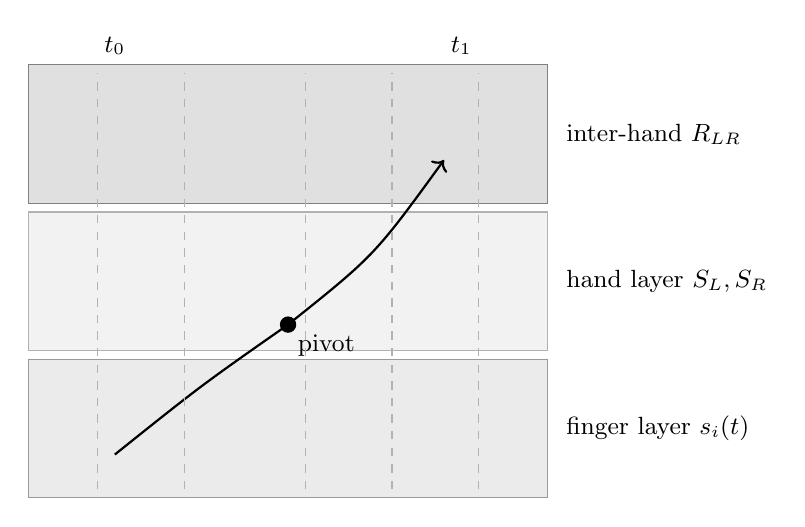
\begin{tikzpicture}[scale=1.1,
  every node/.style={font=\small}]
% Three horizontal planes representing layers
\fill[black!8,draw=black!40]  (-3,-0.8) rectangle (3,0.8);
\fill[black!5,draw=black!30] (-3, 0.9) rectangle (3,2.5);
\fill[black!12,draw=black!50]    (-3, 2.6) rectangle (3,4.2);
% Layer labels
\node[right] at (3.1, 0.0) {finger layer $s_i(t)$};
\node[right] at (3.1, 1.7) {hand layer $S_{L},S_{R}$};
\node[right] at (3.1, 3.4) {inter-hand $R_{LR}$};
% Trajectory rising through layers
\draw[thick,->]
  (-2,-0.3) .. controls (-1,0.5) .. (0,1.2)
            .. controls (1,2.0) .. (1.8,3.1);
\filldraw[black] (0,1.2) circle (2.5pt);
\node[below right] at (0,1.2) {pivot};
% Vertical connector lines
\foreach \x in {-2.2,-1.2,0.2,1.2,2.2}{
  \draw[black!30,dashed] (\x,-0.7) -- (\x,4.1);
}
\node[above] at (-2,4.2) {$t_0$};
\node[above] at (2,4.2)  {$t_1$};
\end{tikzpicture}
\caption{A gesture $G$ as a trajectory through three hierarchical layers of
coordination. The pivot (red) marks a reversal under sustained contact---the
primary structural feature preserved by canonicalisation~\cite{cox2016}.}
\label{fig:layers}
\end{figure}

% -------------------------------------------------------
\section{Gesture Before Symbol: Developmental and Evolutionary Context}

The title of this paper carries a double meaning. In the technical sense
developed throughout, ``gesture before symbol'' refers to the argument
that the relational motor structure of keyboard input precedes and
grounds its symbolic interpretation: $\hat{G}$ is the primary object,
and $\Phi_i(\hat{G})$ is the projection. But the phrase also names an
empirical finding from developmental psychology and evolutionary
anthropology that independently supports the same logical priority.

\subsection{Ontogenetic Precedence}

Research in developmental psychology establishes that communicative
gestures systematically precede symbolic communication in human
infants~\cite{iverson2005gesture}. Between approximately ten and fourteen
months, infants develop deictic gestures---pointing, showing,
reaching---that function as requests or references to objects before
spoken words serve the same function. Crucially, gesture-symbol
combinations (pointing while vocalising) appear before symbol-symbol
combinations (two-word utterances). The gesture does not merely
accompany emerging language; it scaffolds it. The child first establishes
a communicative act through motor action, and the symbol is learned into
that already-functional gestural slot~\cite{goldin2003gesture}.

This developmental sequence has a direct structural parallel in the
framework of this paper. The gesture $\hat{G}$ is not derived from or
dependent on the projection $\Phi_{\mathrm{text}}$. The projection is
learned into the gesture. A child learning the word ``bottle'' already
has a functional pointing gesture that selects the referent; the word
fills that pre-existing communicative role. The canonical gesture
precedes and grounds the symbol in exactly the same sense that $\hat{G}$
precedes $\Phi_i(\hat{G})$.

\subsection{Evolutionary Precedence}

The pattern extends across species. Language-enculturated great apes ---
chimpanzees and bonobos trained to use lexigrams or sign language ---
reliably use reaching and showing gestures to indicate intent well before
they use the corresponding symbolic lexigrams for the same purpose, and
continue to use gestural reference in contexts where symbolic access is
uncertain~\cite{savage2000ape}. This cross-species commonality suggests
that gestural communication is not merely a human developmental
convenience but a phylogenetically earlier and more fundamental mode of
intentional reference. Symbol use is a later, higher-cost layer built
over a gestural substrate that is both evolutionarily older and
cognitively more basic.

Lashley's foundational analysis of serial order in behaviour~\cite{lashley1951}
provides a further dimension of this argument. The problem Lashley
identified---that the surface sequential order of action cannot be
the primary representational format, because sequences are planned and
executed from a pre-sequential hierarchical structure---applies equally
to communicative gesture and to keyboard input. In both cases, the
temporal sequence is a projection of a deeper, non-sequential
organisation.

\subsection{The Shared Logical Structure}

The developmental and evolutionary literature on gesture therefore
provides independent empirical support for the core claim of this paper,
arrived at from a completely different direction. Whether one begins
from developmental observations of infants, comparative observations of
enculturated apes, or the analysis of keyboard event streams, the same
conclusion emerges: gesture is the primary representational object, and
symbol is a downstream projection. The infant's point, the ape's reach,
and the typist's slingshot arc are structurally analogous: each is a
relational motor act that grounds and precedes the symbolic layer built
over it.

This convergence is not coincidental. It reflects a general principle:
any system capable of intentional reference will exhibit gesture before
symbol because gestural acts are computationally and evolutionarily
cheaper, more continuous with basic motor action, and more directly
grounded in the relational structure of the environment. Symbolic
communication is a compression of that gestural substrate, not its
replacement.

% -------------------------------------------------------
\section{The Existing Signal}

\subsection{Touch Typing as Structured Motor Behaviour}

Touch typing is commonly described as a method for efficient text entry,
but this description obscures the structure of the underlying motor
activity. A skilled typist does not operate by selecting keys
independently in sequence. Instead, typing is executed as a coordinated,
distributed process across both hands, in which multiple fingers are
active simultaneously and transitions are planned in advance of discrete
key events.

Each finger operates within a constrained spatial domain defined by
keyboard layout and learned motor habit. These domains are stable over
time: the left pinky reliably services the set \{\texttt{q, a, z}\},
while the right pinky services \{\texttt{p, ;, /}\}. This partitioning
is not merely instructional but becomes internalised as a persistent
mapping between fingers and regions of action. Within these regions,
movement is not discrete but continuous, even though the sensing
apparatus reports only binary contact events.

Crucially, the fingers do not act independently. Skilled typing exhibits
overlapping activation, in which multiple keys are depressed within short
temporal intervals, often with one or more keys held while others are
actuated. These overlaps are not accidental but arise from biomechanical
efficiency: minimising unnecessary lift and repositioning allows for
higher throughput and smoother motion~\cite{schieber2001}.

The result is that, at any given moment, the typist's hands are in a
composite state consisting of multiple active contacts, partial releases,
and anticipatory positioning. This state evolves continuously over time,
forming a trajectory that cannot be reduced to a simple sequence of
independent actions.

\subsection{Temporal Structure: Overlap, Duration, and Release}

The temporal dimension of typing extends beyond the order of key presses.
Each key activation has a duration, and the relative timing of presses
and releases across fingers forms a structured temporal pattern.
Empirically, three features are consistently observable:

\begin{itemize}[leftmargin=2em]
  \item \textbf{Overlap windows.} Keys pressed within short intervals (on
    the order of tens of milliseconds) are often intended as part of a
    single coordinated gesture rather than independent events.
  \item \textbf{Sustained contact vs.\ pass-through.} Some keys are held
    briefly while others are engaged, creating layers of activation that
    persist across transitions.
  \item \textbf{Release ordering.} The order in which fingers disengage
    from keys carries structure, often reflecting the resolution of a
    movement or the completion of a local gesture.
\end{itemize}

These features are stable across repeated executions of the same word or
phrase. A typist does not merely reproduce the same sequence of letters
but tends to reproduce the same timing relationships between
fingers~\cite{monrose2000,gunetti2005}. This temporal structure is
directly perceptible to the typist, manifesting as rhythm, flow, and
coordination rather than as discrete symbolic decisions. Standard input
systems ignore these features entirely, treating only the initial keydown
events as meaningful.

\begin{figure}[h]
\centering
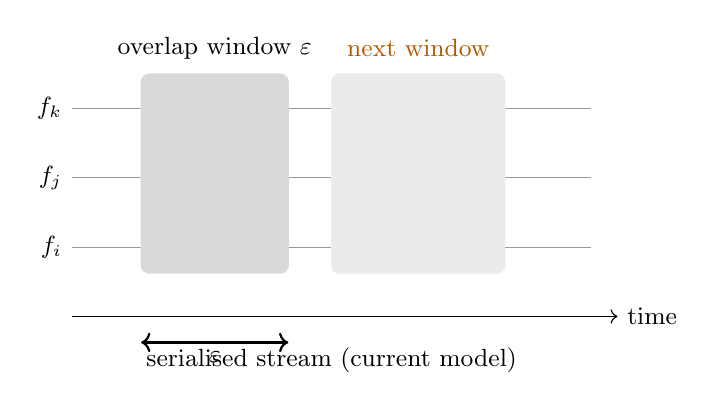
\begin{tikzpicture}[scale=1.1, every node/.style={font=\small}]
% Time axis
\draw[->] (-3,0) -- (3.3,0) node[right]{time};
% Three finger channel axes
\foreach \y/\lbl in {0.8/$f_i$, 1.6/$f_j$, 2.4/$f_k$}{
  \draw[black!40] (-3,\y) -- (3,\y);
  \node[left] at (-3,\y) {\lbl};
}
% Individual serialised events (how current systems see it)
\foreach \x/\y in {-2.0/0.8, -1.5/1.6, -0.8/0.8, 0.2/2.4, 0.9/1.6, 1.8/0.8}{
  \filldraw[black!50] (\x,\y) circle (2pt);
}
\node at (0,-0.5) {serialised stream (current model)};
% Overlap volume (what gesture actually is)
\fill[black!15,rounded corners=3pt]
  (-2.2,0.5) rectangle (-0.5,2.8);
\node[] at (-1.35,3.1) {overlap window $\varepsilon$};
\fill[black!8,rounded corners=3pt]
  (0.0,0.5) rectangle (2.0,2.8);
\node[orange!70!black] at (1.0,3.1) {next window};
\draw[<->,thick] (-2.2,-0.3) -- (-0.5,-0.3);
\node[below] at (-1.35,-0.3) {$\varepsilon$};
\end{tikzpicture}
\caption{Simultaneity as a volumetric overlap region. Serialisation collapses
each shaded volume into a linear sequence, destroying the equivalence
structure $k_i \sim k_j \iff |t_i - t_j| < \varepsilon$.}
\label{fig:overlap}
\end{figure}

\subsection{Biomechanical Constraints and Hand Asymmetry}

The structure of typing is further constrained by the biomechanics of
the hands. The two hands do not contribute symmetrically; they exhibit
distinct and complementary roles:

\begin{itemize}[leftmargin=2em]
  \item \textbf{Anchoring.} One hand maintains a relatively stable
    position or sustained contact while the other executes more dynamic
    movement.
  \item \textbf{Alternation.} Rapid transitions between hands distribute
    load and reduce strain.
  \item \textbf{Convergence and divergence.} The hands move toward or
    away from each other depending on the spatial distribution of
    upcoming keys.
\end{itemize}

These patterns are not consciously controlled but emerge from physical
constraints and the optimisation of movement over time. They are
consistent across typists trained in standard touch-typing technique and
are reinforced through practice. The result is that typing is not simply
a collection of finger actions but a coordinated two-handed system in
which the relationship between the hands encodes additional structure
beyond what any single finger contributes.

\subsection{The Key Switch as a Constraint Accumulator}

A mechanical key switch is not a binary sensor in the ordinary sense. It
is a continuous pressure device with a discrete output threshold. The
actuation point---the position along the travel at which electrical
contact is made---is a singular event in an otherwise continuous
pressure curve. What the firmware receives as a ``keydown'' event is in
reality the crossing of a constraint boundary by a continuous motor
action.

This observation matters for the gesture framework because the
\emph{approach} to actuation carries information. The velocity of the
finger at the moment of contact, the dwell time before actuation, and
the rate of subsequent release all reflect properties of the underlying
gesture. Tactile and clicky switches make the actuation boundary
physically perceptible, which is why experienced typists report different
``feel'' from different switch types---not because the switches change
the symbolic output, but because they change the haptic feedback at the
constraint boundary. In this sense, the key switch acts as a
constraint accumulator: it integrates continuous pressure into a
discrete event, discarding the approach curve in the
process~\cite{juarrero1999}. A
gesture-aware capture layer would ideally record the crossing timestamp
at sub-millisecond resolution alongside the event, preserving as much
of the approach curve as the hardware permits.

\subsection{Stability and Reproducibility of Gesture}

The features described above---overlap, duration, and inter-hand
coordination---are not incidental artefacts but form a stable component
of skilled typing behaviour. A typist repeating a familiar word or phrase
will tend to reproduce similar patterns of overlap between keys, similar
durations of contact for specific fingers, and similar coordination
patterns between the hands. This reproducibility suggests that the
gesture underlying typing is learned as a coherent motor pattern, not
reconstructed from discrete symbolic decisions each time~\cite{lashley1951}.
In other domains, such as musical performance, such patterns are treated
as primary objects of analysis and interpretation. In typing, they are
systematically ignored.

\subsection{Summary}

The act of typing generates a structured signal with the following
properties: concurrent activation across multiple fingers; continuous
temporal variation in duration and release; hierarchical coordination
within and between hands; and constraint-crossing events at the key
switch level. This signal is stable, reproducible, and directly
experienced by the typist. It exists independently of any symbolic
interpretation and precedes the extraction of discrete characters. The
subsequent sections show that current input systems do not merely
simplify this signal but eliminate most of its structure, and that
recovering it requires treating gesture---not symbol---as the primary
object of representation.

% -------------------------------------------------------
\section{What Current Systems Discard}

The flattening performed by standard keyboard interfaces can be
understood as a sequence of projections that systematically eliminate
dimensions of the original motor signal. The result is a representation
that is computationally convenient but information-theoretically
impoverished relative to the gesture that produced it. This section
isolates three dimensions of loss: simultaneity, temporal structure, and
inter-hand relations.

\subsection{Simultaneity and Its Collapse}

Human typing routinely produces near-simultaneous key activations across
multiple fingers. Keystrokes within a window on the order of tens of
milliseconds are perceptually and motorically co-produced, forming what
are effectively micro-chords. Standard input systems do not preserve this
simultaneity. Keyboard controllers scan key matrices sequentially and
emit discrete keydown events that are timestamped and serialised by the
operating system. When multiple keys are actuated within a short
interval, their ordering in the resulting event stream is determined by
scan order, interrupt timing, or driver behaviour rather than by any
meaningful property of the gesture itself.

Formally, let $K = \{k_1, k_2, \ldots\}$ be the set of keydown events,
each with timestamp $t_i$. The original gesture contains equivalence
classes
\[
  k_i \sim k_j \iff |t_i - t_j| < \varepsilon
\]
for some small $\varepsilon$ representing simultaneity. The serialisation
process replaces these classes with a total order:
\[
  k_{i_1} \prec k_{i_2} \prec \cdots \prec k_{i_n},
\]
thereby destroying the equivalence relation. The information loss is
structural: a partially ordered set is reduced to a linear order, and
chordal or synchronous grouping becomes unrepresentable.

At the hardware level, this collapse is exacerbated by the key matrix
rollover limit. Most consumer keyboards report at most six simultaneous
key activations (``6KRO''), with the remainder silently dropped. This
means the full combinatorial space of up to ten simultaneous contacts---the
theoretical maximum for a two-handed touch typist---is not merely
serialised but partially destroyed before the event stream reaches the
operating system. Gaming and mechanical keyboards with true N-key rollover
(NKRO) eliminate this truncation, but the serialisation of simultaneous
events into a total order remains a software-level constraint regardless.

\subsection{Duration and Release Structure}

Each key event has a corresponding release, and the duration between
onset and release encodes a second temporal signal largely independent of
ordering. Conventional text input ignores this structure almost entirely:
keyup events are detected at the hardware level but rarely utilised by
higher-level software. Text entry is defined exclusively in terms of
keydown order, and durations $\Delta t_i = t_i^{\uparrow} -
t_i^{\downarrow}$ are discarded~\cite{killourhy2009,monrose2000}. This
removes hold vs.\ pass-through distinctions, release ordering within a
cluster, and temporal layering across fingers.

The discarding of keyup events is so complete that it is invisible to
most developers. A standard event listener in any major programming
environment exposes \texttt{keydown} and \texttt{keypress} as primary
events, with \texttt{keyup} treated as a cleanup signal of no semantic
significance. This is a design choice, not a physical constraint: the
hardware reports both transitions with equal fidelity. The software stack
then systematically discards half the available signal.

In the gesture formalism introduced below, duration and release are
essential for identifying pivots and segment boundaries; their removal
forces segmentation to be reintroduced artificially via a dedicated
spacebar rather than emerging from the physical gesture.

\subsection{Inter-Hand Relations}

The most consequential loss occurs at the level of inter-hand
coordination. The two hands form a coupled system with stable, learnable
patterns of interaction: convergence, divergence, asymmetric anchoring,
and synchronisation. These patterns align with higher-level structure in
both language and music, yet current input systems provide no
representation of them. Because input is reduced to independent key
events, there is no observable variable corresponding to
\[
  R_{LR}(t) = \mathrm{relation}\bigl(H_L(t),\, H_R(t)\bigr),
\]
where $H_L(t)$ and $H_R(t)$ are the aggregated states of the left and
right hands. This collapse removes an entire layer of structure. While
per-finger events remain observable in degraded form, the geometry of
the hands as a coordinated system is rendered invisible.

\subsection{The Spacebar as Vestigial Organ}

A concrete illustration of the cost of discarding release structure is
the spacebar. In a gesture-first system, word boundaries emerge naturally
from the termination event $t_1 = \inf\{t \mid \forall i,\,
\mathrm{active}_i(t) = 0\}$: the moment all fingers disengage
simultaneously. Full release is an unambiguous physical event that
partitions the gesture stream into units without requiring an additional
key.

The spacebar exists precisely because the serial symbol model cannot use
this signal. Having discarded release structure, the system has no
mechanism for detecting word boundaries and must reintroduce them as an
explicit symbol. The spacebar is therefore not a fundamental input
primitive but an artefact of the lossy compression performed upstream.
In stenographic systems, which preserve chord structure, the stroke
boundary plays an analogous role to full release; the steno writer never
needs a dedicated spacebar~\cite{plover}.

\subsection{Summary of Loss}

The original signal includes concurrent activation across channels,
continuous duration and release structure, and hierarchical coordination
within and between hands. The retained signal includes only ordered
keydown events. Certain structures---pivots defined by reversal under
sustained contact, phrase boundaries defined by coordinated
release---cannot be expressed within the serialised representation. They
are not difficult to detect; they are unrepresentable.

% -------------------------------------------------------
\section{Gesture and Canonical Representation}

\subsection{Finger Channels and Local Domains}

Define the hand as a fixed set of channels $F = \{f_1, \ldots, f_8\}$,
one per finger. Each finger $f_i$ operates over a small local domain
$D_i$ (its constrained key region). At time $t$, each finger has a state
\[
  s_i(t) = \bigl(\mathrm{active}_i(t),\; p_i(t),\; \dot{p}_i(t)\bigr),
\]
where $\mathrm{active}_i(t) \in \{0,1\}$, $p_i(t)$ is the discrete or
interpolated position within $D_i$, and $\dot{p}_i(t)$ is the inferred
direction of migration. The full system state is
$S(t) = \{s_1(t), \ldots, s_8(t)\}$.

\subsection{Hierarchical Structure}

The eight channels are not symmetric. They are organised into two hands:
\[
  H_L = \{f_1, f_2, f_3, f_4\}, \qquad H_R = \{f_5, f_6, f_7, f_8\}.
\]
Hand-level states $S_L(t)$ and $S_R(t)$ are obtained by aggregating
finger states within each hand, extracting the active support set,
dominant direction of motion, and internal coherence (whether fingers are
acting as a unit or independently). The inter-hand relation
$R_{LR}(t) = \langle S_L(t), S_R(t)\rangle$ captures convergence,
divergence, synchronisation, and role asymmetry
$\mathrm{role}(t) \in \{\text{left-anchor},\, \text{right-anchor},\,
\text{co-active}\}$.

A gesture is therefore a time-indexed trajectory through this
three-level structure:
\[
  G = \bigl\{\bigl(S_L(t),\; S_R(t),\; R_{LR}(t)\bigr) \mid t \in [t_0, t_1]\bigr\}.
\]

\subsection{Relational Manifold}

Define derived relational features over $G$:
\begin{align*}
  A(t) &= \{i \mid \mathrm{active}_i(t) = 1\} && \text{(support set)}\\
  \mathrm{sync}(i,j,t) &= \mathrm{active}_i(t) \wedge \mathrm{active}_j(t) && \text{(synchronisation)}\\
  \mathrm{pivot}_i(t) &\iff \dot{p}_i(t^-)\cdot\dot{p}_i(t^+) < 0
    \wedge \mathrm{active}_i(t)=1 && \text{(reversal under contact)}
\end{align*}
The termination event is $t_1 = \inf\{t \mid \forall i,\,
\mathrm{active}_i(t) = 0\}$. The gesture $G$ is a trajectory through a
low-dimensional relational manifold induced by $F$; it is not reducible
to any sequence of key events.

% -------------------------------------------------------
\section{Canonicalisation and Gesture Equivalence}

\subsection{The Canonicalisation Operator}

Define a canonicalisation operator $\mathcal{C}: G \to \hat{G}$ such
that small timing perturbations are discarded while overlap, pivot
structure, and segmentation by full release are preserved. Formally, we
impose a metric $d$ on the raw gesture space such that if
$d(G_1, G_2) < \delta$ then $\mathcal{C}(G_1) = \mathcal{C}(G_2)$, where
$\delta$ is a jitter tolerance threshold calibrated to the polling rate of
the capture hardware. Two raw gestures $G_1$ and $G_2$ are equivalent if
$\mathcal{C}(G_1) = \mathcal{C}(G_2)$. The canonical gesture $\hat{G}$
is the object the user actually learns.

Canonicalisation proceeds hierarchically:
\[
  \mathcal{C} = \mathcal{C}_{\mathrm{inter\text{-}hand}} \circ
                \mathcal{C}_{\mathrm{hand}} \circ
                \mathcal{C}_{\mathrm{finger}}.
\]
At the finger level, timing jitter is suppressed and local pivots are
detected. At the hand level, dominant motion patterns are identified and
fingers are clustered into coherent units. At the inter-hand level,
convergence/divergence and anchor roles are extracted. The hierarchical
composition can be visualised as a sequence of structure-preserving
collapses, each removing distortion while retaining the invariant
geometry of the gesture~\cite{needham1997}.

\subsection{Topological Features}

The canonical gesture preserves three topological features:
\textbf{overlap} (which channels were simultaneously active),
\textbf{pivot} (where reversals occurred under sustained contact), and
\textbf{segmentation} (where full release divided one gesture from the
next). These features are invariant under spatial distortion of the
keyboard, temporal jitter, and changes to output mapping. They constitute
the stable vocabulary the motor system learns.

\subsection{Learnability Condition}

A system is learnable if and only if the canonicalisation is stable under
the distortions the user is likely to encounter. Formally:
\[
  \mathcal{C}(G_{\mathrm{motor}}) = \hat{G}
\]
must hold under spatial distortion of $D_i$, temporal jitter, and
parameter variation in the output mapping. This ensures that motor
equivalence classes coincide with canonical equivalence classes---the
condition under which muscle memory transfers reliably.

\begin{figure}[h]
\centering
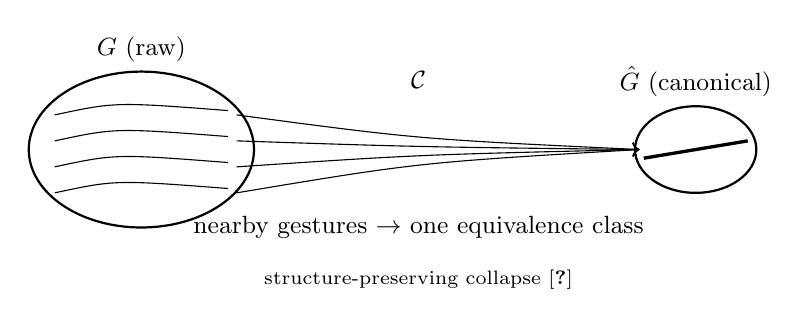
\begin{tikzpicture}[scale=1.1, every node/.style={font=\small}]
% Raw gesture space G (left ellipse, noisy)
\draw[thick] (-3.2,0) ellipse (1.3 and 0.9);
\node[above] at (-3.2,0.9) {$G$ (raw)};
% Several nearby raw trajectories
\foreach \dy in {-0.5,-0.2,0.1,0.4}{
  \draw[thin]
    (-4.2,\dy) .. controls (-3.5,\dy+0.15) .. (-2.2,\dy+0.05);
}
% Canonical gesture space G-hat (right ellipse, clean)
\draw[thick] (3.2,0) ellipse (0.7 and 0.5);
\node[above] at (3.2,0.5) {$\hat{G}$ (canonical)};
% Single canonical trajectory
\draw[very thick]
  (2.6,-0.1) -- (3.8,0.1);
% Fiber collapse arrows
\foreach \dy in {-0.5,-0.2,0.1,0.4}{
  \draw[->]
    (-2.1,\dy) .. controls (0,\dy*0.3) .. (2.55,-0.0);
}
% C label
\node at (0,0.8) {$\mathcal{C}$};
\node at (0,-0.9) {\small nearby gestures $\to$ one equivalence class};
% Needham note
\node[font=\scriptsize] at (0,-1.5)
  {structure-preserving collapse~\cite{needham1997}};
\end{tikzpicture}
\caption{Canonicalisation as a collapse of nearby raw trajectories onto a
single equivalence class. Distortion is removed; topological structure
(overlap, pivot, segmentation) is preserved. The fiber-bundle intuition:
each point in $\hat{G}$ has a fibre of equivalent raw gestures in $G$.}
\label{fig:canonicalisation}
\end{figure}

\begin{figure}[H]
\centering
\small
\begin{minipage}{0.95\textwidth}
\textbf{Reference: Gesture and Canonicalisation}
\medskip

\begin{tabular}{@{}p{3.6cm}p{9.8cm}@{}}
\toprule
\textbf{Object} & \textbf{Definition} \\
\midrule
Finger state & $s_i(t) = (\mathrm{active}_i(t),\;p_i(t),\;\dot{p}_i(t))$ \\
System state & $S(t) = \{s_1(t),\dots,s_8(t)\}$ \\
Gesture & $G = \{S(t)\}_{t\in[t_0,t_1]}$ \\
Support set & $A(t) = \{i\mid\mathrm{active}_i(t)=1\}$ \\
Pivot & $\mathrm{pivot}_i(t)\iff\dot{p}_i(t^-)\cdot\dot{p}_i(t^+)<0\;\wedge\;\mathrm{active}_i=1$ \\
Termination & $t_1=\inf\{t\mid\forall i,\;\mathrm{active}_i(t)=0\}$ \\
Canonicalisation & $\mathcal{C}:G\to\hat{G}$, preserving overlap, pivot, segmentation \\
Learnability & $\mathcal{C}(G_{\mathrm{motor}})=\hat{G}$ stable under jitter and mapping variation \\
\bottomrule
\end{tabular}

\medskip
\textbf{Key structural claim:}
$G \not\equiv \text{sequence}
\;\Longrightarrow\;
\hat{G} = \text{primary object}$.
Typing is a trajectory in a low-dimensional relational manifold; symbols are
projections of that trajectory; canonicalisation extracts the stable topology
of motor knowledge.
\end{minipage}
\caption{Reference sheet: gesture field objects and canonicalisation.
Timing jitter is removed; overlap, pivot, and segmentation are preserved.}
\label{fig:cheat-gesture}
\end{figure}

% -------------------------------------------------------
\section{Gesture Grammar}

\subsection{Gesture Units and Slingshot Arcs}

The canonical gesture decomposes into pivot-centred units:
\[
  \hat{G} = (\gamma_1, \gamma_2, \ldots, \gamma_n),
\]
where each $\gamma_k$ is a \emph{slingshot arc}: a convergence phase, a
pivot, and a divergence phase,
\[
  \gamma_k = (\mathrm{approach},\; \mathrm{pivot},\; \mathrm{release}).
\]
Pivot points are gesturally prominent: they are the moments of maximal
constraint, where one or more fingers reverse direction while remaining
in contact. They correspond naturally to syllabic peaks in speech and
harmonic anchors in music.

The slingshot arc also provides a formal basis for why keystroke dynamics
work as biometric identifiers~\cite{monrose2000,gunetti2005}. Biometric
systems typically treat timing as a hidden feature; the present framework
promotes it to a first-class structural component. The pivot density and
arc shape of a gesture are as characteristic as a signature, and for the
same reason: they reflect the compiled motor patterns of an individual
user.

\begin{figure}[h]
\centering
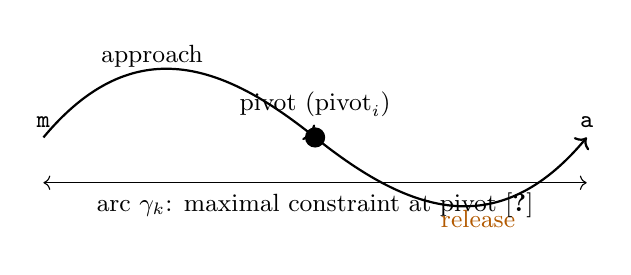
\begin{tikzpicture}[scale=1.15, every node/.style={font=\small}]
% Approach arc
\draw[thick,->]
  (-3,0) .. controls (-2,1.2) and (-1,0.8) .. (0,0);
% Release arc
\draw[thick,->]
  (0,0) .. controls (1,-0.8) and (2,-1.2) .. (3,0);
% Pivot point
\filldraw[black] (0,0) circle (3pt);
\node[above=4pt] at (0,0) {pivot ($\mathrm{pivot}_i$)};
% Labels
\node[] at (-1.8,0.9) {approach};
\node[orange!70!black] at (1.8,-0.9) {release};
\node[above] at (-3,0) {\texttt{m}};
\node[above] at (3,0)  {\texttt{a}};
% Constraint annotation
\draw[<->] (-3,-0.5) -- (3,-0.5);
\node[below] at (0,-0.5) {arc $\gamma_k$: maximal constraint at pivot~\cite{juarrero1999}};
\end{tikzpicture}
\caption{Slingshot arc $\gamma_k = (\mathrm{approach}, \mathrm{pivot}, \mathrm{release})$.
The pivot is the moment of maximal constraint: fingers reverse direction while
remaining in contact. This is not a symbolic event but a bodily one~\cite{cox2016}.}
\label{fig:slingshot}
\end{figure}

\subsection{Composition}

Gesture units compose by concatenation across release boundaries or by
sharing a pivot. The word \emph{machine}, for instance, decomposes into
three slingshot arcs: \texttt{m}$\leftrightarrow$\texttt{a},
\texttt{a}$\leftrightarrow$\texttt{ch}, and
\texttt{i}$\leftrightarrow$\texttt{n}$\leftrightarrow$\texttt{e}, where
each pivot letter serves simultaneously as the endpoint of one arc and
the origin of the next. This decomposition is not imposed on the gesture
but emerges from its physical structure.

\subsection{Anchor--Pivot Asymmetry}

A refinement of the slingshot arc concerns the role asymmetry between
hands. In many gestures, one hand acts as an anchor---maintaining a
stable or slowly evolving position---while the other hand executes the
high-frequency movement that carries most of the local information. The
anchor hand provides the \emph{context} within which the pivot hand's
movements are interpreted. Formalising this:

\[
  \gamma_k = \bigl(\mathrm{anchor}(H_L \text{ or } H_R),\;
               \mathrm{trajectory}(H_{\neg\mathrm{anchor}}),\;
               \mathrm{pivot}\bigr)
\]

This structure is directly analogous to the relationship between bass and
melody in tonal music: the anchoring voice establishes harmonic context,
and the melodic voice moves within it~\cite{cox2016}. It also explains why some
word-initial chords feel natural and others do not---the hand assignment
at the onset of each arc constrains what subsequent movements are
biomechanically smooth.

% -------------------------------------------------------
\section{Projection Framework}

\subsection{Projection Functors}

Let $\hat{\mathcal{G}}$ denote the space of canonical gestures. Define
projection functors
\begin{align*}
  \Phi_{\mathrm{text}}   &: \hat{\mathcal{G}} \to \Sigma^* \\
  \Phi_{\mathrm{music}}^{\,\theta} &: \hat{\mathcal{G}} \to \mathcal{M} \\
  \Phi_{\mathrm{visual}} &: \hat{\mathcal{G}} \to \mathcal{V}
\end{align*}
where $\Sigma^*$ is the space of strings, $\mathcal{M}$ is a
pitch-time structure, and $\mathcal{V}$ is a space of visual forms.
Each functor depends only on $\hat{G}$, not on the raw event stream.

The following commutative diagram illustrates the relationship between
the raw gesture, canonicalisation, and projection:

\[
\begin{tikzcd}[column sep=3em, row sep=2.5em]
  G \arrow[r, "\mathcal{C}"] \arrow[dr, dashed, "\Phi_i \circ \mathcal{C}"']
    & \hat{G} \arrow[d, "\Phi_i"] \\
    & \mathcal{O}_i
\end{tikzcd}
\]

The dashed arrow confirms that whether one first canonicalises and then
projects, or composes both operations directly from the raw stream, the
result is the same output $\mathcal{O}_i$. This commutativity is the
formal expression of the claim that canonical gesture is the correct
intermediate representation: it does not lose information that matters
for projection.

\subsection{Metric Independence}

Let $\theta$ be a mapping parameter (pitch range, tuning, text
dictionary). Then $\Phi_{\mathrm{music}}^{\,\theta}(\hat{G})$ varies
with $\theta$ while $\hat{G}$ remains fixed. This formalises the design
principle: the mapping layer may change freely; the gesture grammar must
remain invariant. A single learned motor vocabulary can project into
multiple modalities without relearning.

\subsection{Core Claim}

Meaning is a function of gesture equivalence classes, not of symbol
sequences:
\[
  \mathrm{meaning} : \hat{\mathcal{G}} \to \text{output domain}.
\]
Text, music, and visual form are projections of a shared underlying
structure. The gesture is the primary object; the projections are
secondary.

% -------------------------------------------------------
\section{Admissibility as a Meta-Constraint Structure}

The projection framework defines mappings from canonical gesture space to
output domains. A projection specifies \emph{how} a gesture is rendered;
but it does not specify \emph{whether} the result is structurally valid.
This distinction motivates a further layer: admissibility.

\subsection{The Admissibility Functional}

Define an admissibility functional
\[
  \mathcal{A} : \hat{\mathcal{G}} \times \{\Phi_i\} \to \mathbb{R}_{\ge 0}
\]
A projected output is admissible if
\[
  \mathcal{A}(\hat{G}, \Phi_i) > \tau
\]
for some threshold $\tau$. Admissibility captures conditions such as:
whether a gesture closes coherently under projection (e.g., a gesture
that maps to a fragment of a word rather than a complete word has low
admissibility under $\Phi_{\mathrm{text}}$); whether the projected
output is globally consistent (e.g., a musical phrase that violates the
current harmonic constraint has low admissibility under
$\Phi_{\mathrm{music}}$); and whether the equivalence class is
unambiguous (e.g., a gesture that maps to multiple equally plausible
words has reduced admissibility because the projection is not injective
at that point).

\subsection{The Admissibility Log}

Rather than treating admissibility as a static predicate, we define the
admissibility log as the temporal trace of this evaluation:
\[
  \mathcal{L} = \bigl\{ \bigl(\hat{G}_t,\; \Phi_i,\; \mathcal{A}_t,\; \epsilon_t\bigr) \bigr\}_{t}
\]
where $\hat{G}_t$ is the canonical gesture at time $t$, $\Phi_i$ is the
active projection, $\mathcal{A}_t$ is the admissibility score, and
$\epsilon_t$ is an obstruction term encoding failure of closure. The
obstruction captures incompatibility between local gesture segments under
projection, failure of global consistency (non-gluable outputs), and
ambiguity across equivalence classes.

\subsection{Non-Reductive Character}

Unlike the projection functors $\Phi_i$, which reduce the
dimensionality of the gesture representation, the admissibility structure
is non-reductive: it introduces additional structure rather than
collapsing it, encodes global constraints across time, and tracks the
history of constraint satisfaction and failure. It is therefore better
understood as a functor into a category of constraint-evaluated objects
rather than into an output domain:
\[
  \mathcal{A} : \hat{\mathcal{G}} \to \mathbf{Constr}
\]
where objects in $\mathbf{Constr}$ are pairs $(\hat{G}, \Phi_i)$
equipped with coherence conditions.

\subsection{Extended Diagram}

The full three-stage structure can be represented as:

\[
\begin{tikzcd}[column sep=3em, row sep=2.5em]
  G \arrow[r, "\mathcal{C}"]
    & \hat{G} \arrow[r, "\Phi_i"] \arrow[dr, "\mathcal{A}"']
    & \mathcal{O}_i \\
    &  & \mathbf{Constr}
\end{tikzcd}
\]

Canonicalisation identifies what the gesture \emph{is}; projection
specifies how it is \emph{rendered}; admissibility evaluates whether the
rendering is \emph{valid}. Together they form a complete pipeline from
raw motor input to validated symbolic or musical output.

\begin{figure}[h]
\centering
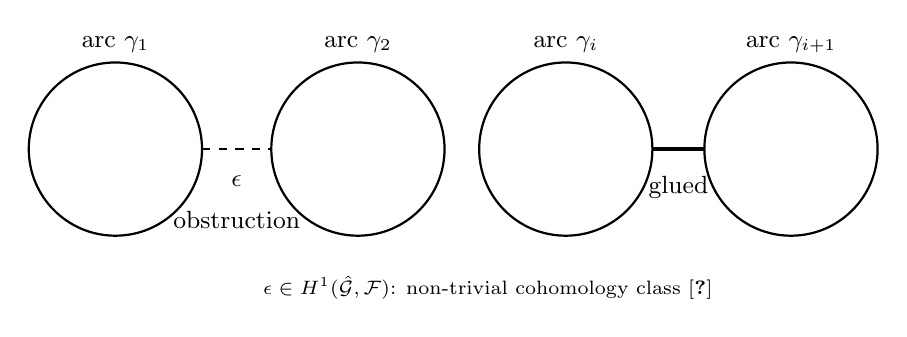
\begin{tikzpicture}[scale=1.1, every node/.style={font=\small}]
% Two local gesture arc patches
\draw[thick] (-3,0) circle (1.0);
\draw[thick] (-0.2,0) circle (1.0);
\node[above] at (-3,1.0)  {arc $\gamma_1$};
\node[above] at (-0.2,1.0) {arc $\gamma_2$};
% Attempted gluing (dashed red gap)
\draw[thick,dashed] (-2.0,0) -- (-1.2,0);
\node[below] at (-1.6,-0.2) {$\epsilon$};
\node[below] at (-1.6,-0.6) {\small obstruction};
% A successfully glued pair (right side)
\draw[thick] (2.2,0) circle (1.0);
\draw[thick] (4.8,0) circle (1.0);
\draw[very thick] (3.2,0) -- (3.8,0);
\node[below] at (3.5,-0.2) {glued};
\node[above] at (2.2,1.0)  {arc $\gamma_i$};
\node[above] at (4.8,1.0)  {arc $\gamma_{i+1}$};
% Juarrero constraint note
\node[font=\scriptsize] at (1.3,-1.6)
  {$\epsilon \in H^1(\hat{\mathcal{G}},\mathcal{F})$: non-trivial cohomology class~\cite{juarrero2002}};
\end{tikzpicture}
\caption{Failure of local gesture arcs to glue into a globally admissible
structure (left) versus successful gluing (right). The obstruction $\epsilon$
is not a local error but a global topological invariant.}
\label{fig:obstruction}
\end{figure}

\begin{figure}[H]
\centering
\small
\begin{minipage}{0.95\textwidth}
\textbf{Reference: Projection and Admissibility}
\medskip

\begin{tabular}{@{}p{3.6cm}p{9.8cm}@{}}
\toprule
\textbf{Object} & \textbf{Definition} \\
\midrule
Projection functor & $\Phi_i:\hat{\mathcal{G}}\to\mathcal{O}_i$ \quad (text $\Sigma^*$, music $\mathcal{M}$, visual $\mathcal{V}$) \\
Admissibility & $\mathcal{A}:(\hat{G},\Phi_i)\to\mathbb{R}_{\ge0}$;\quad admissible iff $\mathcal{A}(\hat{G},\Phi_i)>\tau$ \\
Admissibility log & $\mathcal{L}=\{(\hat{G}_t,\Phi_i,\mathcal{A}_t,\epsilon_t)\}_t$ \\
Obstruction & $\epsilon\in H^1(\hat{\mathcal{G}},\mathcal{F})$: non-trivial cohomology class \\
Metric independence & $\Phi_{\mathrm{music}}^\theta(\hat{G})$ varies with $\theta$; $\hat{G}$ invariant \\
Commutativity & $\Phi_i\circ\mathcal{C}$ depends only on $\hat{G}$, not raw stream \\
\bottomrule
\end{tabular}

\medskip
\textbf{Two-layer structure:} projection reduces dimensionality; admissibility adds
structure and records constraint history.
\quad\textbf{Sheaf interpretation:} global coherence exists iff $\epsilon=0$;
failure of meaning $\equiv$ non-gluable local structure.
\end{minipage}
\caption{Reference sheet: projection functors, admissibility functional, and obstruction.}
\label{fig:cheat-proj}
\end{figure}

% -------------------------------------------------------
\section{Amplitwist Cascades: Recursive Geometric Evaluation}

The admissibility framework introduced above defines a constraint layer
over canonical gestures and their projections. It does not yet specify
the \emph{internal geometry} through which a gesture is evaluated prior
to projection. This section introduces the amplitwist cascade as the
geometric mechanism underlying that evaluation~\cite{needham1997}.

The central claim is that a canonical gesture $\hat{G}$ does not map
directly to an output domain. Instead, it induces a trajectory in an
epistemic manifold $M$ equipped with RSVP fields $(\Phi, \vec{v}, S)$,
and is evaluated through a sequence of recursive deformations of that
manifold. The cascade is not a pipeline between different spaces; it is
progressive warping of the same manifold under accumulated Lie action.

\subsection{The Base Amplitwist Operator}

On the RSVP manifold $M$, let $\Phi : M \to \mathbb{R}$ be the scalar
constraint-density field, $\vec{v} : M \to TM$ the plenum velocity
field, and $S : M \to \mathbb{R}_+$ the entropy field. Define the base
amplitwist operator:
\[
  \mathcal{A}(\vec{x}) =
  \|\vec{v}(\vec{x})\| \cdot
  \exp\!\left(
    i \cdot \arccos\!\left(
      \frac{\vec{v}(\vec{x}) \cdot \nabla\Phi(\vec{x})}
           {\|\vec{v}(\vec{x})\|\,\|\nabla\Phi(\vec{x})\| + \varepsilon}
    \right)
  \right),
\]
where $\varepsilon > 0$ ensures numerical stability. This operator
decomposes into two geometrically distinct components:
\begin{align*}
  \rho(\vec{x}) &= \|\vec{v}(\vec{x})\| && \text{(amplitude: intensity of conceptual flow)}\\
  \theta(\vec{x}) &= \arccos\!\left(
    \frac{\vec{v}\cdot\nabla\Phi}{\|\vec{v}\|\,\|\nabla\Phi\|+\varepsilon}
  \right) && \text{(phase: alignment with semantic gradient)}
\end{align*}
The amplitwist encodes a local rotation and scaling in the tangent space
of $M$, generalising the complex derivative interpretation of conformal
maps~\cite{needham1997} to the RSVP setting.

\subsection{Recursive Lie-Algebraic Deformations}

Let $\mathfrak{so}(n)$ denote the Lie algebra of skew-symmetric
transformations on $M$. Each semantic layer introduces an infinitesimal
deformation $T_j \in \mathfrak{so}(n)$ scaled by $\epsilon_j \in
\mathbb{R}$. Define the accumulated deformation:
\[
  \mathfrak{R}_k(\vec{x}) = \vec{x} + \sum_{j=1}^k \epsilon_j T_j(\vec{x}).
\]
This is not a sequence of mappings between distinct spaces but a
progressive warping of $M$ that preserves differentiable structure. The
composition $\mathfrak{R}_k$ defines a flow on $M$ generated by
$\mathfrak{so}(n)$:
\[
  M \;\mapsto\; \mathfrak{R}_1(M) \;\mapsto\; \cdots \;\mapsto\; \mathfrak{R}_k(M).
\]

\subsection{Layered Amplitwist Evaluation}

The amplitwist at layer $k$ is evaluated at the deformed point
$\mathfrak{R}_k(\vec{x})$ with entropy weighting:
\[
  \mathcal{A}^{(k)}(\vec{x}) =
  w_k(\vec{x}) \cdot \mathcal{A}\!\bigl(\mathfrak{R}_k(\vec{x})\bigr),
  \qquad
  w_k(\vec{x}) = e^{-\lambda S(\vec{x})}.
\]
Deformation accumulates forward; entropy suppresses amplitude
multiplicatively. The cascade $\mathcal{A}^{(0)}, \mathcal{A}^{(1)},
\ldots, \mathcal{A}^{(k)}$ is a recursive evaluation over a continuously
deformed manifold in which amplitude, phase, and entropy jointly
determine the stability of interpretation.

\begin{figure}[H]
\centering
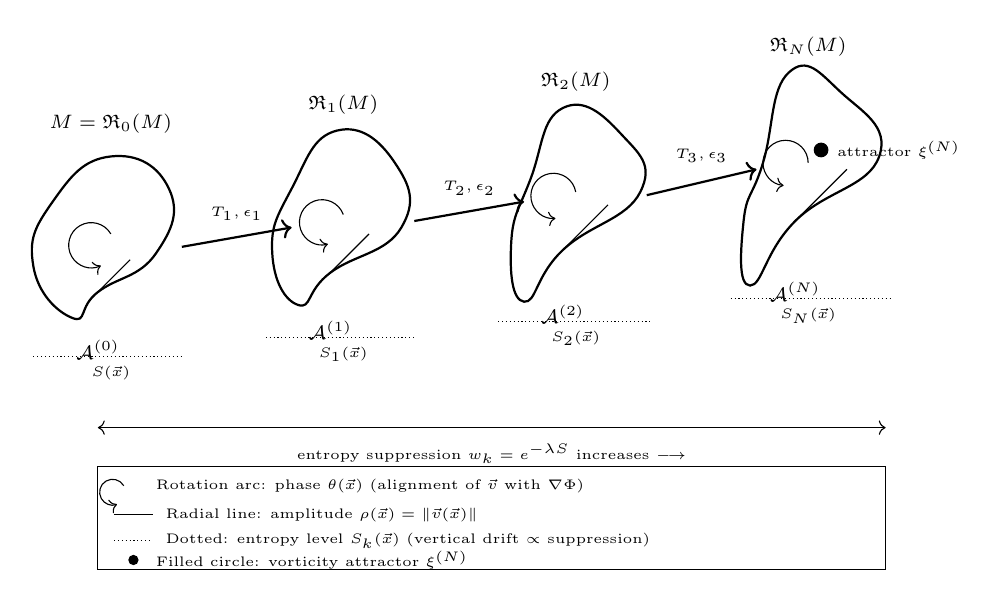
\begin{tikzpicture}[scale=0.82, every node/.style={font=\scriptsize},
  every path/.style={draw=black}]

%% Stage 0
\begin{scope}[xshift=0cm, yshift=0cm]
  \draw[thick] plot[smooth cycle, tension=0.85]
    coordinates {(0,0)(0.9,0.6)(1.1,1.6)(0.2,2.1)(-0.7,1.4)(-1.0,0.4)(-0.4,-0.4)};
  \draw[->] (0.2,0.9) arc[start angle=30,end angle=295,radius=0.35];
  \draw[thin] (0,0) -- (0.5,0.5);
  \node[above] at (0.2,2.3) {$M = \mathfrak{R}_0(M)$};
  \node[below] at (0,-0.6) {$\mathcal{A}^{(0)}$};
  \draw[thin,densely dotted] (-1.0,-1.0) -- (1.3,-1.0);
  \node[below,font=\tiny] at (0.2,-1.0) {$S(\vec{x})$};
\end{scope}

%% Arrow 1
\draw[->,thick] (1.3,0.7) -- (3.0,1.0);
\node[above,font=\tiny] at (2.15,0.95) {$T_1,\epsilon_1$};

%% Stage 1
\begin{scope}[xshift=3.6cm, yshift=0.3cm]
  \draw[thick] plot[smooth cycle, tension=0.85]
    coordinates {(0,0)(1.1,0.7)(1.0,1.7)(0.1,2.2)(-0.6,1.3)(-0.9,0.3)(-0.5,-0.5)};
  \draw[->] (0.2,0.9) arc[start angle=20,end angle=285,radius=0.35];
  \draw[thin] (0,0) -- (0.6,0.6);
  \node[above] at (0.2,2.3) {$\mathfrak{R}_1(M)$};
  \node[below] at (0,-0.6) {$\mathcal{A}^{(1)}$};
  \draw[thin,densely dotted] (-1.0,-1.0) -- (1.3,-1.0);
  \node[below,font=\tiny] at (0.2,-1.0) {$S_1(\vec{x})$};
\end{scope}

%% Arrow 2
\draw[->,thick] (4.9,1.1) -- (6.6,1.4);
\node[above,font=\tiny] at (5.75,1.35) {$T_2,\epsilon_2$};

%% Stage 2
\begin{scope}[xshift=7.2cm, yshift=0.65cm]
  \draw[thick] plot[smooth cycle, tension=0.85]
    coordinates {(0,0)(1.2,0.9)(0.9,1.8)(0.0,2.2)(-0.5,1.1)(-0.8,0.1)(-0.6,-0.8)};
  \draw[->] (0.2,0.9) arc[start angle=10,end angle=275,radius=0.35];
  \draw[thin] (0,0) -- (0.7,0.7);
  \node[above] at (0.2,2.3) {$\mathfrak{R}_2(M)$};
  \node[below] at (0,-0.7) {$\mathcal{A}^{(2)}$};
  \draw[thin,densely dotted] (-1.0,-1.1) -- (1.4,-1.1);
  \node[below,font=\tiny] at (0.2,-1.1) {$S_2(\vec{x})$};
\end{scope}

%% Arrow 3
\draw[->,thick] (8.5,1.5) -- (10.2,1.9);
\node[above,font=\tiny] at (9.35,1.85) {$T_3,\epsilon_3$};

%% Stage 3
\begin{scope}[xshift=10.8cm, yshift=1.1cm]
  \draw[thick] plot[smooth cycle, tension=0.85]
    coordinates {(0,0)(1.3,1.0)(0.7,2.0)(-0.1,2.3)(-0.5,0.9)(-0.8,0.0)(-0.7,-1.0)};
  \draw[->] (0.2,0.9) arc[start angle=0,end angle=265,radius=0.35];
  \draw[thin] (0,0) -- (0.8,0.8);
  \filldraw[black] (0.4,1.1) circle (3pt);
  \node[right,font=\tiny] at (0.5,1.1) {attractor $\xi^{(N)}$};
  \node[above] at (0.2,2.4) {$\mathfrak{R}_N(M)$};
  \node[below] at (0,-0.8) {$\mathcal{A}^{(N)}$};
  \draw[thin,densely dotted] (-1.0,-1.2) -- (1.5,-1.2);
  \node[below,font=\tiny] at (0.2,-1.2) {$S_N(\vec{x})$};
\end{scope}

%% Entropy suppression axis
\draw[<->,thin] (0,-2.1) -- (12.2,-2.1);
\node[below,font=\tiny] at (6.1,-2.2)
  {entropy suppression $w_k = e^{-\lambda S}$ increases $\longrightarrow$};

%% Legend box
\draw[thin] (0,-2.7) rectangle (12.2,-4.3);
\draw[->] (0.4,-3.0) arc[start angle=30,end angle=290,radius=0.2];
\node[right,font=\tiny] at (0.75,-3.0)
  {Rotation arc: phase $\theta(\vec{x})$ (alignment of $\vec{v}$ with $\nabla\Phi$)};
\draw[thin] (0.25,-3.45) -- (0.85,-3.45);
\node[right,font=\tiny] at (0.9,-3.45)
  {Radial line: amplitude $\rho(\vec{x}) = \|\vec{v}(\vec{x})\|$};
\draw[thin,densely dotted] (0.25,-3.85) -- (0.85,-3.85);
\node[right,font=\tiny] at (0.9,-3.85)
  {Dotted: entropy level $S_k(\vec{x})$ (vertical drift $\propto$ suppression)};
\filldraw[black] (0.55,-4.15) circle (2pt);
\node[right,font=\tiny] at (0.75,-4.15)
  {Filled circle: vorticity attractor $\xi^{(N)}$};

\end{tikzpicture}
\caption{Amplitwist cascade: recursive deformation of manifold $M$ under
Lie-generated flows $\mathfrak{R}_k$, with layer-$k$ amplitwist
$\mathcal{A}^{(k)}(\vec{x}) = w_k(\vec{x})\,\mathcal{A}(\mathfrak{R}_k(\vec{x}))$.
Rotation arcs encode phase $\theta$; radial lines encode amplitude $\rho$;
dotted lines mark entropy levels; vertical drift encodes suppression.
The filled circle marks the emergent attractor $\xi^{(N)}$~\cite{juarrero1999}.}
\label{fig:cascade-formal}
\end{figure}

\subsection{Emergent Vorticity and Attractors}

Let $\hat{\vec{v}}^{(N)}$ denote the velocity field transported through
the cascade. Define the emergent vorticity:
\[
  \xi^{(N)}(\vec{x}) = \|\nabla \times \hat{\vec{v}}^{(N)}(\vec{x})\|.
\]
Regions of high vorticity are stable attractors in the epistemic
manifold---points at which recursive deformation and amplitwist alignment
converge. A gesture induces a trajectory whose cascade evaluation either
converges to an attractor (high admissibility) or disperses (low
admissibility). Admissibility can therefore be reinterpreted as:
\[
  \mathcal{A}(\hat{G}, \Phi_i) \;\sim\;
  \text{stability of } \mathcal{A}^{(N)} \text{ under cascade flow}.
\]
Theorem~3.1 of the RSVP programme guarantees that $\xi^{(N)}$ converges
when $\epsilon_j < \epsilon_{\mathrm{crit}}$~\cite{juarrero1999}.

\subsection{Integration with Gesture and Projection}

The gesture-first framework defines:
\[
  G \xrightarrow{\mathcal{C}} \hat{G} \xrightarrow{\Phi_i} \mathcal{O}_i.
\]
The amplitwist cascade inserts an internal geometric evaluation stage:
\[
  \hat{G} \;\longrightarrow\;
  \mathfrak{R}_k(\hat{G}) \;\longrightarrow\;
  \mathcal{A}^{(k)} \;\longrightarrow\;
  \Phi_i.
\]
Canonical gesture $\hat{G}$ specifies initial conditions on $M$;
recursive deformation $\mathfrak{R}_k$ defines the trajectory in
epistemic space; amplitwist $\mathcal{A}^{(k)}$ evaluates local
alignment and intensity; projection $\Phi_i$ renders the resulting
structure. Admissibility then operates over the entire cascade:
\[
  \mathcal{A}(\hat{G}, \Phi_i)
  \;\equiv\;
  \mathrm{coherence}\bigl(\{\mathcal{A}^{(k)}\}_k\bigr).
\]

The key objects of the cascade are summarised in
Table~\ref{tab:cascade}.

\begin{table}[H]
\centering
\renewcommand{\arraystretch}{1.35}
\begin{tabular}{@{}p{3.0cm}p{6.0cm}p{4.8cm}@{}}
\toprule
\textbf{Object} & \textbf{Definition} & \textbf{Role} \\
\midrule
Base operator &
  $\mathcal{A}(\vec{x}) = \|\vec{v}\|\exp(i\theta)$ &
  Amplitude from velocity; phase from alignment \\[4pt]
Recursive layer &
  $\mathfrak{R}_k = \vec{x} + \sum_j\epsilon_j T_j(\vec{x})$, $T_j\in\mathfrak{so}(n)$ &
  Lie-algebraic deformation \\[4pt]
Layer-$k$ amplitwist &
  $\mathcal{A}^{(k)} = w_k\,\mathcal{A}(\mathfrak{R}_k)$, $w_k=e^{-\lambda S}$ &
  Entropy-weighted evaluation \\[4pt]
Vorticity &
  $\xi^{(N)} = |\nabla\times\hat{\vec{v}}^{(N)}|$ &
  Emergent attractor structure \\
\bottomrule
\end{tabular}
\caption{Key objects of the amplitwist cascade.}
\label{tab:cascade}
\end{table}

\subsection{Conceptual Closure}

The amplitwist cascade provides a unifying interpretation of the
framework developed in this paper. It replaces static representation
with recursive deformation: meaning is not read off from a gesture but
emerges through successive geometric transformations. Entropy suppresses
amplitwist magnitude, biasing the system toward low-energy attractors.
Admissibility reduces to geometric stability: a projection is valid if
and only if the cascade converges to a stable attractor.

The cascade integrates with the broader RSVP programme: the scalar,
vector, and entropy fields $(\Phi, \vec{v}, S)$ define the local
geometry; the amplitwist operator encodes alignment within that geometry;
and the cascade describes how local structure propagates across scales.
It is not an additional component of the system but the internal
geometry through which gesture, projection, and admissibility become
coherent~\cite{juarrero1999,needham1997,cox2016}.

Interpretation is not a mapping from symbol to meaning, but a trajectory
through a recursively deformed geometric field whose stable attractors
constitute what is recognised as meaning.

% -------------------------------------------------------
\section{CLIO as Gradient Flow on the Amplitwist Cascade}

CLIO (Cognitive Loop via In-Situ Optimization) is a framework introduced
by Cheng, Broadbent, and Chappell~\cite{cheng2025clio} in which large
language models self-formulate approaches to problems, adapt when
self-confidence is low, and allow external observation and correction of
internal reasoning states. The key features of CLIO---open uncertainty
representation, graph-structured belief states, and scientist
interjectability---align structurally with the gesture-first framework
developed in this paper. In the gesture setting, the ``scientist'' is
the user, the ``reasoning process'' is the amplitwist cascade, and
``steerability'' is precisely the intervention parameter
$\Delta t_{\mathrm{ctrl}}$ of Section~\ref{sec:control}.

We reinterpret CLIO here as a gradient flow on the cascade energy,
connecting its adaptive self-confidence mechanism to the geometric
stability of the amplitwist attractor. The original CLIO paper operates
over LLM belief states; the present interpretation generalises this to
any recursive geometric evaluation system, of which gesture-driven
projection is a specific instance.

The amplitwist cascade defines the geometry of interpretation. It does
not yet specify how the system \emph{evolves} toward admissibility. This
role is fulfilled by the gradient flow on the cascade energy.

\subsection{Energy Functional}

Let $\{\mathcal{A}^{(k)}(\vec{x})\}_{k=0}^N$ be the amplitwist cascade.
Define the cascade energy:
\[
  \mathcal{E}(\vec{x}) =
  \sum_{k=0}^N \alpha_k \left(
    \|\nabla\theta^{(k)}(\vec{x})\|^2 +
    \beta\,\|\nabla\rho^{(k)}(\vec{x})\|^2
  \right) + \mu S(\vec{x}),
\]
where $\rho^{(k)}$ and $\theta^{(k)}$ are the amplitude and phase of
$\mathcal{A}^{(k)}$, $\alpha_k$ weights cascade layers, $\beta$ balances
amplitude vs.\ phase smoothness, and $\mu$ penalises entropy. This
functional measures incoherence across the cascade: rapid spatial
variation in phase or amplitude corresponds to misalignment; high entropy
corresponds to instability.

\subsection{Gradient Flow Dynamics}

The gradient flow on $\mathcal{E}$ is:
\[
  \frac{d\vec{x}}{dt} = -\nabla\mathcal{E}(\vec{x}).
\]
This implements a continuous repair process: given a gesture $\hat{G}$,
the system evolves its position in the epistemic manifold until the
amplitwist cascade becomes stable. It moves toward regions of aligned
phase (low $\|\nabla\theta\|$), smooths amplitude variation (low
$\|\nabla\rho\|$), and descends toward lower entropy (low $S$).

\subsection{Relation to Control Resolution}

The control resolution parameter $\Delta t_{\mathrm{ctrl}}$ determines
how this flow is realised. In high-intervention regimes
($\Delta t_{\mathrm{ctrl}} \to 0$), the user perturbs $\vec{x}$ directly
during the flow---analogous to the scientist interjectability feature of
CLIO~\cite{cheng2025clio}. In low-intervention regimes, the system integrates the
flow to a fixed point before exposing the result. Both regimes follow the
same gradient flow but differ in how frequently external intervention
modifies the trajectory.

\subsection{Fixed Points and Admissibility}

A point $\vec{x}^*$ is a fixed point if $\nabla\mathcal{E}(\vec{x}^*) = 0$.
These correspond to stable attractors of the amplitwist cascade. A
gesture $\hat{G}$ is admissible if its induced trajectory under this flow
converges to a fixed point:
\[
  \text{admissibility}
  \;\Longleftrightarrow\;
  \text{convergence of gradient flow.}
\]
Admissibility is therefore not a binary predicate but a dynamical
property of the system.

% -------------------------------------------------------
\section{Amplitwist Loss as an Admissibility Functional}

The admissibility functional $\mathcal{A}(\hat{G}, \Phi_i)$ has thus far
been defined abstractly. The amplitwist cascade provides a natural
instantiation in terms of cross-system alignment.

\subsection{Definition of Amplitwist Loss}

Let $\mathcal{A}^{(k)}_{\mathrm{sys}}$ denote the cascade induced by a
system and $\mathcal{A}^{(k)}_{\mathrm{ref}}$ a reference cascade
(human gesture dynamics or a canonical semantic field). Define:
\[
  \mathcal{L}_A =
  \sum_{k=0}^N
  \left\|
    \mathcal{A}^{(k)}_{\mathrm{sys}}(\vec{x}) -
    \mathcal{A}^{(k)}_{\mathrm{ref}}(\vec{x})
  \right\|^2.
\]
This measures discrepancy at the level of recursive geometric evaluation,
not final output.

\subsection{Decomposition by Amplitude and Phase}

Expanding $\mathcal{A}^{(k)} = \rho^{(k)}e^{i\theta^{(k)}}$:
\[
  \mathcal{L}_A =
  \sum_{k=0}^N
  \left(
    \|\rho^{(k)}_{\mathrm{sys}} - \rho^{(k)}_{\mathrm{ref}}\|^2
    + \gamma\|\theta^{(k)}_{\mathrm{sys}} - \theta^{(k)}_{\mathrm{ref}}\|^2
  \right),
\]
where $\gamma$ balances amplitude and phase alignment. This separates two
failure modes: \textbf{amplitude mismatch} (incorrect intensity) and
\textbf{phase mismatch} (misalignment with semantic gradients).

\subsection{Admissibility as Bounded Loss}

Admissibility is now quantitative:
\[
  \mathcal{A}(\hat{G}, \Phi_i) > \tau
  \;\Longleftrightarrow\;
  \mathcal{L}_A < \varepsilon.
\]
A projection is admissible not because it satisfies symbolic constraints
but because its recursive geometric evaluation aligns with the reference
cascade.

\subsection{Relation to CLIO}

The gradient flow and the loss are dual:
\[
  \nabla\mathcal{E} \to 0
  \;\Rightarrow\;
  \mathcal{L}_A \to 0.
\]
Convergence of internal dynamics produces alignment with the reference
cascade. Together, CLIO (internal repair) and $\mathcal{L}_A$ (external
alignment) complete the admissibility structure: the cascade defines the
geometry of interpretation, the gradient flow defines the dynamics of
repair, and the amplitwist loss defines the criterion of alignment.

% -------------------------------------------------------
\section{Variational Principle for the Amplitwist Cascade}

The amplitwist cascade can be derived from a variational principle.
Rather than treating the recursive operators and amplitwists as
definitional, we regard them as extrema of an action functional.

\subsection{Cascade Energy}

Define:
\[
  \mathcal{E}_{\mathrm{cas}}
  = \sum_{k=0}^{N} \int_M
  \left[
    \alpha_k \|\nabla\mathcal{A}^{(k)}\|^2
    + \beta_k \|\mathcal{A}^{(k)} - \mathcal{A}^{(k-1)}\|^2
    + \mu_k S|\mathcal{A}^{(k)}|^2
  \right] d\mu,
\]
(with the second term omitted for $k=0$). Writing $\mathcal{A}^{(k)} =
\rho^{(k)}e^{i\theta^{(k)}}$, the gradient term decomposes as:
\[
  \|\nabla\mathcal{A}^{(k)}\|^2
  = \|\nabla\rho^{(k)}\|^2
  + (\rho^{(k)})^2\|\nabla\theta^{(k)}\|^2.
\]
The three terms penalise local roughness, layer discontinuity, and
entropy-weighted amplitude respectively.

\subsection{Full Action}

\[
  \mathcal{S}_{\mathrm{amp}}
  = \int_{t_0}^{t_1}
  \left(
    \mathcal{E}_{\mathrm{cas}}
    + \mathcal{E}_{\mathrm{RSVP}}
    + \mathcal{E}_{\mathrm{adm}}
  \right) dt,
\]
where the RSVP field energy is:
\[
  \mathcal{E}_{\mathrm{RSVP}}
  = \int_M
  \left[
    a_\Phi\|\nabla\Phi\|^2
    + a_v\|\nabla\vec{v}\|^2
    + a_S\|\nabla S\|^2
    + b\,S\|\vec{v}\|^2
  \right] d\mu,
\]
and the admissibility energy penalises obstruction:
\[
  \mathcal{E}_{\mathrm{adm}} = \int_M \|\epsilon(\vec{x})\|^2\,d\mu.
\]

\subsection{Stationary Condition}

The realised interpretation is obtained by extremising the action:
\[
  \delta\mathcal{S}_{\mathrm{amp}} = 0,
\]
which yields stationarity conditions with respect to $\Phi$, $\vec{v}$,
$S$, and $T_j$ simultaneously. These express the same principle at four
levels: scalar salience, vector flow, entropy modulation, and recursive
deformation must jointly stabilise.

\subsection{Central Identity}

The variational formulation gives the cascade a field-theoretic status:
meaning is not a lookup but a constrained relaxation. The core principle
of the paper can now be stated as a single equation:
\[
  \boxed{
    \mathrm{meaning}
    = \operatorname*{arg\,ext}_{X,\{T_j\}}
    \mathcal{S}_{\mathrm{amp}}[X,\{T_j\}]
  }
\]
Meaning is the stationary structure of an entropy-weighted,
gesture-driven amplitwist cascade~\cite{juarrero1999,needham1997}.

\begin{figure}[H]
\centering
\small
\begin{minipage}{0.95\textwidth}
\textbf{Reference: Control, CLIO, and Amplitwist Optimisation}
\medskip

\begin{tabular}{@{}p{4.0cm}p{9.4cm}@{}}
\toprule
\textbf{Object} & \textbf{Definition} \\
\midrule
Control resolution & $\Delta t_{\mathrm{ctrl}}$: minimum interval for gesture to modify $x(t)$ \\
Tool regime & $\Delta t_{\mathrm{ctrl}}\to 0$: continuous coupling, external repair \\
Agent regime & large $\Delta t_{\mathrm{ctrl}}$: single-step mapping, internal repair \\
CLIO energy & $\mathcal{E}=\sum_k\alpha_k(\|\nabla\theta^{(k)}\|^2+\beta\|\nabla\rho^{(k)}\|^2)+\mu S$ \\
Gradient flow & $d\vec{x}/dt = -\nabla\mathcal{E}(\vec{x})$\quad (CLIO~\cite{cheng2025clio} as descent) \\
Fixed point & $\nabla\mathcal{E}=0\;\Rightarrow\;$stable interpretation \\
Amplitwist loss & $\mathcal{L}_A=\sum_k\|\mathcal{A}^{(k)}_{\mathrm{sys}}-\mathcal{A}^{(k)}_{\mathrm{ref}}\|^2$ \\
Admissibility & $\mathcal{L}_A<\varepsilon\;\Longleftrightarrow\;$admissible \\
Variational identity & $\mathrm{meaning}=\operatorname{arg\,ext}_{X,\{T_j\}}\mathcal{S}_{\mathrm{amp}}[X,\{T_j\}]$ \\
\bottomrule
\end{tabular}

\medskip
\textbf{System closure:}
$\hat{G}\to\text{cascade}\to\text{CLIO flow}\to\text{fixed point}\to\Phi_i$.
CLIO provides internal repair; $\mathcal{L}_A$ provides external alignment;
$\Delta t_{\mathrm{ctrl}}$ determines coupling.
\textbf{Key principle:}
Meaning $=$ stable fixed point of constrained geometric flow.
\end{minipage}
\caption{Reference sheet: control resolution, CLIO gradient dynamics, amplitwist loss,
and the variational identity.}
\label{fig:cheat-control}
\end{figure}

\begin{figure}[H]
\centering
\small
\begin{minipage}{0.95\textwidth}
\textbf{Unified RSVP--Amplitwist--Admissibility System}
\medskip

\begin{tabular}{@{}p{3.8cm}p{9.6cm}@{}}
\toprule
\textbf{Layer} & \textbf{Content} \\
\midrule
RSVP base fields & $X=(\Phi,\vec{v},S)$: scalar potential, vector flow, entropy \\
Gesture coupling & $\hat{G}\to\vec{v}(\vec{x},t)$: gesture as boundary condition on flow \\
Amplitwist & $\mathcal{A}(\vec{x})=\|\vec{v}\|e^{i\theta}$: local rotation-scaling in $TM$ \\
Cascade & $\mathcal{A}^{(k)}=e^{-\lambda S}\mathcal{A}(\mathfrak{R}_k)$: entropy-weighted recursive deformation \\
Vorticity & $\xi^{(N)}=|\nabla\times\hat{v}^{(N)}|$: emergent attractor structure \\
Projection & $\Phi_i:\hat{\mathcal{G}}\to\mathcal{O}_i$: rendering into output domain \\
Admissibility & $\mathcal{A}_{\mathrm{adm}}\sim\int|\nabla\theta^{(N)}|^2+\mu S$: coherence measure \\
Constraint closure & $\epsilon=0\;\Longleftrightarrow\;$global coherence \\
\bottomrule
\end{tabular}

\medskip
\textbf{Full system flow:}
$\hat{G}\to\vec{v}\to\mathcal{A}^{(k)}\to\xi^{(N)}\to\Phi_i\to\mathcal{A}_{\mathrm{adm}}$.

\medskip
\textbf{Core identity:}
\[
  \text{Meaning}
  = \text{entropy-weighted stable flow structure}
  = \operatorname*{arg\,ext}_{X,\{T_j\}}\mathcal{S}_{\mathrm{amp}}
\]
\end{minipage}
\caption{Unified reference: RSVP fields, amplitwist cascade, gesture input, and admissibility
as a single constrained dynamical system.}
\label{fig:cheat-unified}
\end{figure}

% -------------------------------------------------------
\section{Hardware and System Constraints}

\subsection{Keyboard Matrix Limitations}

Standard keyboards scan key matrices at rates of approximately one to
eight kilohertz, with hardware debounce filters that introduce latency on
the order of milliseconds. N-key rollover is absent on many consumer
devices, limiting the number of simultaneously reported keys to six or
fewer. These constraints mean that concurrent gesture structure is
collapsed at the point of capture, before any software layer has an
opportunity to interpret it.

The USB HID protocol, which governs how keyboards communicate with host
systems, was designed around a 125\,Hz polling rate (8\,ms per report),
though USB high-speed mode supports 1000\,Hz (1\,ms). Most operating
systems default to 125\,Hz unless explicitly configured otherwise. At
this polling rate, two keystrokes separated by less than 8\,ms are
indistinguishable from simultaneous. The simultaneity equivalence window
$\varepsilon$ in our formalism is therefore bounded below by the polling
period: any implementation must account for this hardware floor when
calibrating $\delta$ in the canonicalisation metric.

\subsection{Required Capabilities}

Capturing the gesture signal described in this paper does not require a
new form factor. It requires: true N-key rollover across all keys;
high-resolution timestamps on keydown and keyup events (sub-millisecond
resolution); and access to raw keyup events at the application level.
These capabilities exist in current gaming and mechanical keyboard
hardware with QMK-compatible controllers (such as the Teensy series
running at 1000\,Hz polling), but are not exposed by standard input
pipelines.

Developers working in this space should note that \texttt{evdev} on
Linux provides raw key event timestamps at kernel-level resolution and
exposes both keydown and keyup events with equal fidelity. The
\texttt{libevdev} C library and \texttt{python-evdev} wrapper provide
direct access to this stream without the semantic filtering imposed by
higher-level input frameworks. On macOS, the \texttt{CGEventTap}
interface provides analogous low-level access. On Windows,
\texttt{SetWindowsHookEx} with \texttt{WH\_KEYBOARD\_LL} captures
low-level keyboard events including keyup with system timestamps,
though the timestamp resolution depends on the timer resolution set via
\texttt{timeBeginPeriod}.

\subsection{Minimal Instrument Specification}

A gesture-capable input layer requires: a capture module delivering raw
timestamped keydown and keyup events; a channel mapping from physical
keys to finger identities; a feature extractor computing overlap,
duration, direction, and inter-hand relations; a canonicalisation
pipeline implementing $\mathcal{C}$; and a pluggable projection layer
implementing $\Phi_i$. No new hardware is required. The instrument is a
software layer that reads what the hands are already producing.

% -------------------------------------------------------
\section{Relationship to Existing Systems}

Existing input systems can be situated within the gesture framework by
examining how much of the relational signal each preserves. A useful
prior step is to observe that these systems differ along two independent
axes: \emph{continuous vs.\ symbolic} (whether the signal is a spatial
path or a discrete command element) and \emph{low-dimensional
vs.\ high-dimensional} (the size of the space the input navigates).
Trace keyboards are continuous and low-dimensional: the finger draws a
path through a flat letter grid~\cite{zhai2012}. Symbolic systems such
as Vim, Bash, or Emacs are discrete and high-dimensional: each keypress
or chord is an element in a large combinatorial space. These two axes
are orthogonal, and the positions systems occupy on them predict which
dimensions of gesture they preserve and which they discard.

A second structural observation concerns the relationship between chorded
and sequential input. Chords and key sequences are not categorically
different; they are dual encodings of the same underlying structure---a
prefix tree, or trie, over possible intentions (i.e., a hierarchical
decision structure in which each node narrows the space of valid next
actions). A chord selects a node in that tree in parallel; a sequence
walks a path to the same node one step at a time. Systems such as
Spacemacs make this equivalence explicit: the binding
\texttt{SPC\,f\,s} (space, file, save) is a sequential traversal of the
same hierarchy that a single chord might compress into simultaneity. GUI
menus, shell directory traversal (\texttt{cd /usr/local/bin}), and
chorded keybindings are all encodings of hierarchical navigation; what
differs is whether the tree is externalised in the display or
internalised in motor memory. The \texttt{which-key} plugin in Emacs and
Spacemacs is precisely a mechanism for rendering the implicit trie
visible on demand---collapsing the tree back into a menu when the user
needs to explore rather than execute. This trie structure is also present
in the gesture grammar of Section~6: pivot-centred arcs are the nodes,
and composition by shared pivot is traversal through the tree.

Standard typing collapses the gesture entirely to ordered keydown
events: $G \to \{k_{i_1} \prec k_{i_2} \prec \cdots\}$~\cite{mackenzie2002}.
Stenography preserves simultaneity within a stroke but discards duration
and release ordering~\cite{plover}. Swype-style trace keyboards preserve
single-finger spatial trajectory but discard multi-finger parallelism and
inter-hand structure~\cite{zhai2012}. Musical instruments preserve
duration and timing but treat inter-finger coordination as implicit in
the acoustic output rather than as an explicit signal. General gesture
recognisers have explored trajectory-based representations at the level
of single-pointer input~\cite{wobbrock2007}, but without the
multi-channel relational structure described here.

No existing system treats inter-hand relational structure as a primary
signal. The present framework is distinguished by defining meaning at the
level of inter-channel coordination rather than individual channel events.

The developmental and evolutionary literature reviewed in Section~2
provides a further axis of comparison. Existing input systems, without
exception, assume the symbol as primitive and treat gesture as an encoding
problem: how do we get from motor action to symbolic output as efficiently
as possible? The gesture-before-symbol framework inverts this. In
developmental terms, input system design has been proceeding as though
children learn to point by first learning words---when in fact the
arrow runs the other way. The correct design question is not ``how do we
recognise the symbol the user intends?'' but ``how do we preserve enough
of the gestural structure that the symbol can be unambiguously projected
from it?''~\cite{iverson2005gesture,goldin2003gesture}.

% -------------------------------------------------------
\section{Implications}

If gesture is the primary object, several consequences follow. First, a
single learned motor vocabulary can project simultaneously into text,
music, and visual form without requiring separate training for each
modality---the same gesture that types a word produces a musical phrase
and a visual contour. Second, skill transfer between typing and musical
performance becomes structurally grounded rather than merely analogical:
both exploit the same hierarchical relational structure~\cite{schieber2001}.
This explains why some people find the transition between piano and
keyboard intuitive: the underlying relational manifold is the same; only
$\Phi$ is swapped. Third, the design space for input systems expands from
symbol-entry optimisation to gesture-representation fidelity, shifting
the engineering question from \emph{how do we recognise keystrokes
faster?} to \emph{how much of the gesture do we preserve?} Isomorphic
keyboard designs, which seek layout-invariant chord
shapes~\cite{lumatone}, represent one existing step in this direction,
though they remain committed to fixed pitch mappings rather than the
dynamic projection framework described here.

A fourth consequence bears on how intelligence is distributed in
human-computer systems. Much current discourse assumes that intelligence
must be centralised in a general-purpose agent---a model that interprets
inputs, reasons over them, and produces outputs. The gesture-first
framework suggests a different picture. If a well-designed interface
preserves the relational structure of the user's intention and projects
it faithfully into multiple domains, then a large fraction of what is
normally attributed to the intelligence of the \emph{system} is better
understood as intelligence of the \emph{coupling}. Tools like Vim, Bash,
or a well-designed trace keyboard are not intelligent in the agent sense;
they are intelligent in the sense that they preserve and amplify the
structure the user brings. The keyboard in this framework is not a
switchboard but a high-bandwidth sensor whose full signal has never been
read. The present framework extends this principle: by treating gesture
as primary and projection as secondary, it locates expressive power in
the trained motor system of the user rather than in any centralised
interpreter. The interface becomes not a black box that translates
intention into output, but a transparent medium that preserves the
structure of gesture across modalities.

% -------------------------------------------------------
\section{Intervention and Control: Tools and Agents as a Continuum}
\label{sec:control}

The distinction between ``tools'' and ``agents'' is commonly framed in
terms of autonomy. Within the gesture-first framework, this distinction
can be expressed more precisely as a property of the \emph{control loop}
linking gesture, projection, and admissibility.

Given a canonical gesture $\hat{G}$ and a projection $\Phi_i$, the
system produces an output trajectory $x(t)$. The admissibility functional
$\mathcal{A}$ evaluates this trajectory and yields an obstruction signal
$\epsilon_t$ when coherence fails. The critical question is how this
obstruction is resolved---and by whom.

\subsection{External Repair (High-Intervention Systems)}

In high-intervention systems, the repair loop remains external. The user
observes $\epsilon_t$ and updates the gesture:
\[
  \hat{G}_{t+1} = \mathrm{repair}(\hat{G}_t,\; \epsilon_t).
\]
Projection is applied incrementally, and admissibility is enforced
through continuous user intervention. The system dynamics are tightly
coupled to gesture:
\[
  x(t+\delta t) = F\bigl(x(t),\; \hat{G}_{[t,\, t+\delta t]}\bigr).
\]
Editors, shells, and direct manipulation interfaces operate in this
regime. The user retains control over the trajectory at fine temporal
resolution, and admissibility is achieved through iterative refinement
rather than autonomous internal computation.

\subsection{Internal Repair (Low-Intervention Systems)}

In low-intervention systems, the repair loop is internalised. A gesture
$\hat{G}$ is treated as an initial condition, and the system applies an
internal process that attempts to resolve admissibility without further
input:
\[
  x(t_1) = F\bigl(x(t_0),\; \hat{G}\bigr).
\]
The user observes only the final outcome and may intervene only by
aborting or restarting. Large language models, batch compilers, and
automated pipelines exemplify this regime. Note that the internalisation
of the repair loop does not increase the expressive power of the
projection---it relocates where constraint satisfaction occurs.

\subsection{Control Resolution}

The distinction between these regimes is not categorical but continuous.
Let $\Delta t_{\mathrm{ctrl}}$ denote the minimum interval at which
gesture can modify the evolving trajectory $x(t)$. High-intervention
systems satisfy
\[
  \Delta t_{\mathrm{ctrl}} \to 0,
\]
while low-intervention systems exhibit large $\Delta t_{\mathrm{ctrl}}$,
approaching a single-step mapping from initial condition to final output.
The critical parameter is not the complexity of the internal model but
the temporal resolution at which the user's gesture remains coupled to
system dynamics.

\subsection{Coupling Strength and Expressive Power}

Expressive power is not solely a property of $\Phi_i$ but of the
\emph{coupling} between $\hat{G}$ and system dynamics. When
$\Delta t_{\mathrm{ctrl}}$ is small, the relational structure of
$\hat{G}$ is continuously reflected in $x(t)$, and admissibility is
achieved through direct manipulation. When $\Delta t_{\mathrm{ctrl}}$ is
large, the mapping $\hat{G} \mapsto x(t_1)$ is mediated by internal
dynamics, and the original gesture structure is partially obscured.

This explains an otherwise puzzling phenomenon: systems with minimal
internal modelling can feel more powerful than systems with substantial
internal modelling. The difference is not capability but coupling. A
tightly coupled simple system preserves the gesture structure all the
way to the output; a loosely coupled complex system substitutes its own
internal dynamics for the user's intent.

\subsection{Interpretation}

Tools and agents are not fundamentally distinct classes. They are points
along a continuum defined by $\Delta t_{\mathrm{ctrl}}$ and the location
of admissibility repair. The gesture-first framework suggests that
increasing capability does not require increasing autonomy. It requires
preserving the user's ability to intervene in the evolving trajectory
and to participate in the repair process that enforces admissibility.

The design question shifts from ``how autonomous should the system be?''
to ``at what temporal and structural resolution should gesture remain
coupled to system dynamics?''

\begin{figure}[h]
\centering
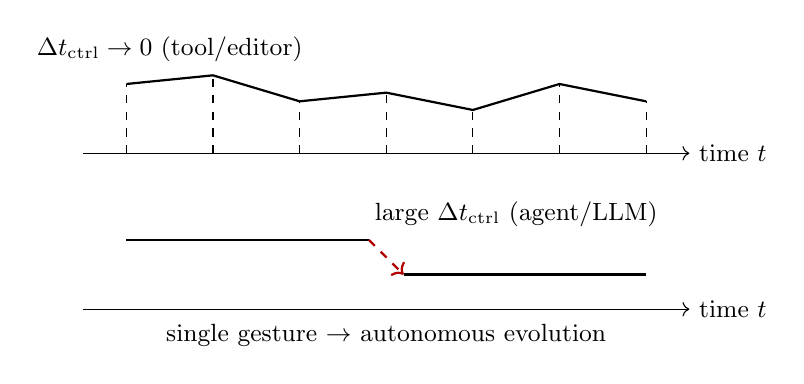
\begin{tikzpicture}[scale=1.1, every node/.style={font=\small}]
% Time axis
\draw[->] (-3.5,0) -- (3.5,0) node[right]{time $t$};
\draw[->] (-3.5,-1.8) -- (3.5,-1.8) node[right]{time $t$};
% Continuous coupling (tool)
\draw[thick]
  (-3,0.8) -- (-2,0.9) -- (-1,0.6) -- (0,0.7) -- (1,0.5) -- (2,0.8) -- (3,0.6);
\draw[thin,dashed]
  (-3,0) -- (-3,0.8)  (-2,0) -- (-2,0.9)  (-1,0) -- (-1,0.6)
  (0,0) -- (0,0.7)  (1,0) -- (1,0.5)  (2,0) -- (2,0.8)  (3,0) -- (3,0.6);
\node[] at (-2.5,1.2) {$\Delta t_{\mathrm{ctrl}}\to 0$ (tool/editor)};
% Discrete jump (agent)
\draw[thick]
  (-3,-1.0) -- (-0.2,-1.0);
\draw[thick,red!70!black,->,dashed]
  (-0.2,-1.0) -- (0.2,-1.4);
\draw[thick]
  (0.2,-1.4) -- (3,-1.4);
\node[] at (1.5,-0.7) {large $\Delta t_{\mathrm{ctrl}}$ (agent/LLM)};
\node[] at (-0.0,-2.1) {\small single gesture $\to$ autonomous evolution};
\end{tikzpicture}
\caption{Continuous coupling (tool regime, top) versus discrete jump (agent
regime, bottom). In the tool regime, gesture can modify $x(t)$ at fine
resolution; in the agent regime, $\hat{G}$ becomes an initial condition
for an autonomous process the user cannot steer mid-flight.}
\label{fig:control}
\end{figure}

% -------------------------------------------------------
\section{Future Directions}

\subsection{Optimal Control Resolution}

The introduction of $\Delta t_{\mathrm{ctrl}}$ as a continuous parameter
suggests a research programme for optimising control resolution in
gesture-coupled systems. Fully autonomous systems and fully manual tools
may both be suboptimal extremes: the former sacrifice expressive coupling
for convenience; the latter place the full repair burden on the user.
Hybrid systems in which admissibility repair is partially external and
partially internal may offer a more favourable balance. Characterising
the Pareto frontier between responsiveness and autonomy---and identifying
which gesture structures are most sensitive to control resolution---is an
open problem.

\subsection{Admissibility Log as a Design Primitive}

The admissibility log $\mathcal{L}$ introduced in Section~8 records the
temporal evolution of $\epsilon_t$ across gesture--projection pairs. A
natural extension is to expose this log to the user as an interactive
surface: a mechanism by which the history of constraint satisfaction and
failure becomes visible and manipulable. In such a system, the user would
intervene not only in the gesture itself but in the dynamics of
admissibility evaluation, steering the trajectory toward coherence at the
meta-level.

This extends the gesture-first framework from representation and
projection to a third layer: the user's relationship to the constraint
structure governing valid output. Whether this layer can be made
navigable through gesture---treating admissibility itself as a space to
explore---is an open question with implications for programming
environments, musical improvisation systems, and structured writing tools.

\subsection{Esoteric Input Languages}

The gesture grammar introduced in Section~6 is defined over the
biomechanical constraints of standard keyboards. A natural extension is
to explore alternative constraint structures: non-standard keyboard
layouts such as Dvorak or Colemak alter the finger-domain partition
without changing the relational manifold; chorded keyboards such as
stenographic systems alter the simultaneity structure; and isomorphic
instruments such as the Lumatone alter the pitch-mapping geometry.

More speculatively, the framework opens the possibility of intentionally
designed ``esoteric'' input languages---gesture grammars where the
canonical equivalence classes are defined not by phonological or
musical convention but by arbitrary structural criteria. Just as esoteric
programming languages explore the boundary between computation and symbol
manipulation, gesture languages could explore the boundary between motor
control and semantic production. The canonicalisation operator
$\mathcal{C}$ would remain invariant; only the projection $\Phi_i$
would change, mapping the same gesture vocabulary into a novel output
domain.

\subsection{Cryptographic Applications}

The stability and individuality of gesture patterns under canonicalisation
has a direct application in authentication and cryptographic key
derivation. Keystroke dynamics as a biometric have been studied
primarily at the level of timing sequences~\cite{killourhy2009,monrose2000};
the present framework suggests that the richer relational structure of
canonical gestures---overlap patterns, pivot density, anchor-hand
asymmetry, and inter-hand synchronisation---could provide substantially
higher entropy for biometric identification or continuous authentication.

Because $\hat{G}$ is defined over topological features rather than raw
timestamps, canonicalisation introduces a structural inversion with
cryptographic implications. On the eavesdropper's side, timing-based
side-channel attack yields only an equivalence class under $\mathcal{C}$
rather than a unique signature: the jitter tolerance $\delta$ acts as a
privacy parameter, collapsing nearby timing signatures into a single
canonical form. On the authenticator's side, the same equivalence
structure increases internal distinctiveness, because two users with
similar timing profiles may nonetheless produce distinct canonical
gestures if their overlap patterns, pivot structure, or anchor-hand
asymmetry differ. The system trades raw timing precision for higher-level
structural entropy. Developing a cryptographically grounded treatment of
gesture-based authentication---including formal bounds on the entropy of
$\hat{G}$ and the privacy loss introduced by $\mathcal{C}$---is a
natural direction for future work.

\subsection{Gesture Space as a Dynamical System}

The present framework treats $G$ as a trajectory, but has not fully
analysed the space of gestures as a dynamical system in its own right.
A natural extension is to define a flow on gesture space:
\[
  \frac{dG}{dt} = \mathcal{F}(G,\; u(t)),
\]
where $u(t)$ is the motor input signal and $\mathcal{F}$ encodes
biomechanical and coupling constraints. Under this view, the gesture
space acquires attractors (commonly repeated words, phrases, or musical
motifs), repellers (biomechanically difficult configurations), and stable
limit cycles (rhythmic patterns in music or typing). Learning then
corresponds to the convergence of motor trajectories toward the basin of
attraction of a canonical gesture class, and expertise is characterised
by reduced variance around that attractor. The canonicalisation operator
$\mathcal{C}$ can be interpreted as a projection onto the attractor
manifold, and the learnability condition of Section~5 becomes a
condition on the width of that manifold relative to the noise in $u(t)$.

This dynamical framing connects the gesture-first framework to the
broader programme in which trajectories---not states---are the primary
objects of analysis. The RSVP amplitwist cascade formalises this
connection precisely. Define the base amplitwist operator on the
canonical gesture manifold:
\[
  \mathcal{A}(\hat{G}) = \|\vec{v}(\hat{G})\|\cdot
  \exp\!\left(i\;\arccos\frac{\vec{v}(\hat{G})\cdot\nabla\Phi(\hat{G})}
  {\|\vec{v}\|\,\|\nabla\Phi\|+\varepsilon}\right),
\]
where $\vec{v}$ is the RSVP velocity field, $\Phi$ is the scalar
constraint-density field, and $\varepsilon>0$ ensures stability. The
phase angle $\theta = \arccos(\cdots)$ encodes the misalignment between
conceptual velocity and the semantic salience gradient; the amplitude
$\|\vec{v}\|$ encodes the magnitude of the gesture's kinetic energy.

Recursive semantic layers $\mathfrak{R}_k$ deform the base manifold via
accumulated Lie-algebraic rotations:
\[
  \mathfrak{R}_k(\hat{G}) = \hat{G} + \sum_{j=1}^{k}\epsilon_j T_j(\hat{G}),
  \qquad T_j \in \mathfrak{so}(n),
\]
and the layer-$k$ amplitwist is evaluated at the deformed point with an
entropy suppression weight:
\[
  \mathcal{A}^{(k)}(\hat{G}) = w_k(\hat{G})\cdot\mathcal{A}(\mathfrak{R}_k(\hat{G})),
  \qquad w_k = e^{-\lambda S(\hat{G})}.
\]
As $k$ increases, the manifold warps under the accumulated Lie action,
and emergent vorticity $\xi^{(N)} = |\nabla\times\hat{v}|$ identifies
stable attractor regions---the gesture-space analogue of common words,
phrases, or musical motifs. Theorem~3.1 of the RSVP programme
establishes that $\xi^{(N)}$ converges when $\epsilon_j < \epsilon_{\mathrm{crit}}$,
guaranteeing that the cascade reaches a stable attractor rather than
diverging~\cite{juarrero1999}.

\begin{figure}[H]
\centering
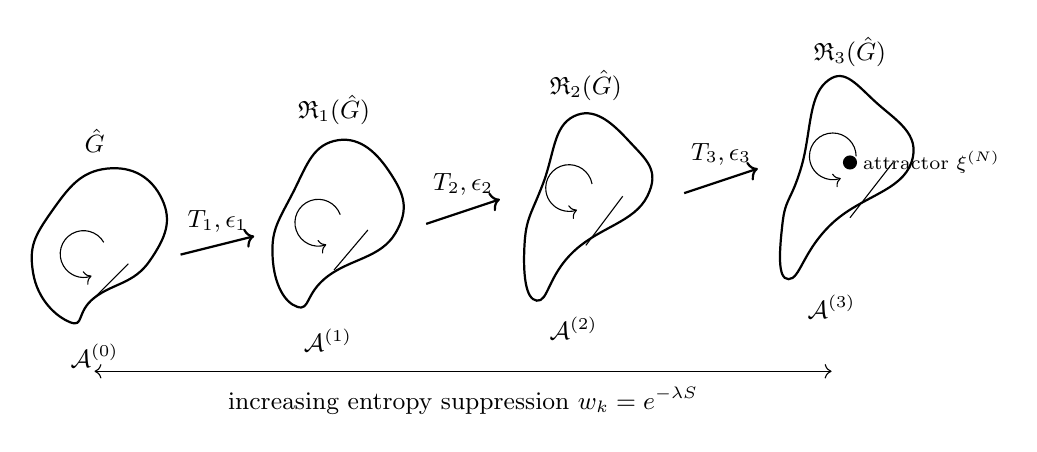
\begin{tikzpicture}[scale=0.78, every node/.style={font=\small},
  every path/.style={draw=black}]

%% Manifold 0: base
\draw[thick]
  plot[smooth cycle, tension=0.85]
  coordinates {(0,0)(0.9,0.6)(1.1,1.6)(0.2,2.1)(-0.7,1.4)(-1.0,0.4)(-0.4,-0.4)};
\node[above] at (0,2.2) {$\hat{G}$};
\node[below] at (0,-0.6) {$\mathcal{A}^{(0)}$};
% Phase arc (rotation indicator)
\draw[->] (0.15,0.9) arc[start angle=30, end angle=290, radius=0.38];
% Amplitude radial
\draw[thin] (0,0) -- (0.55,0.55);

%% Arrow 1
\draw[->,thick] (1.4,0.7) -- (2.6,1.0);
\node[above] at (2.0,0.9) {$T_1,\epsilon_1$};

%% Manifold 1: first deformation (shifted right and slightly up)
\begin{scope}[xshift=3.8cm, yshift=0.35cm]
\draw[thick]
  plot[smooth cycle, tension=0.85]
  coordinates {(0,0)(1.1,0.7)(1.0,1.7)(0.1,2.2)(-0.6,1.3)(-0.9,0.3)(-0.5,-0.5)};
\node[above] at (0.1,2.3) {$\mathfrak{R}_1(\hat{G})$};
\node[below] at (0,-0.7) {$\mathcal{A}^{(1)}$};
\draw[->] (0.2,1.0) arc[start angle=20, end angle=290, radius=0.38];
\draw[thin] (0.1,0.1) -- (0.65,0.75);
\end{scope}

%% Arrow 2
\draw[->,thick] (5.4,1.2) -- (6.6,1.6);
\node[above] at (6.0,1.5) {$T_2,\epsilon_2$};

%% Manifold 2: second deformation
\begin{scope}[xshift=7.8cm, yshift=0.75cm]
\draw[thick]
  plot[smooth cycle, tension=0.85]
  coordinates {(0,0)(1.2,0.9)(0.9,1.8)(0.0,2.2)(-0.5,1.1)(-0.8,0.1)(-0.6,-0.8)};
\node[above] at (0.2,2.3) {$\mathfrak{R}_2(\hat{G})$};
\node[below] at (0,-0.9) {$\mathcal{A}^{(2)}$};
\draw[->] (0.3,1.1) arc[start angle=10, end angle=290, radius=0.38];
\draw[thin] (0.2,0.1) -- (0.8,0.9);
\end{scope}

%% Arrow 3
\draw[->,thick] (9.6,1.7) -- (10.8,2.1);
\node[above] at (10.2,2.0) {$T_3,\epsilon_3$};

%% Manifold 3: third deformation (highest)
\begin{scope}[xshift=12.0cm, yshift=1.2cm]
\draw[thick]
  plot[smooth cycle, tension=0.85]
  coordinates {(0,0)(1.3,1.0)(0.7,2.0)(-0.1,2.3)(-0.5,0.9)(-0.8,0.0)(-0.7,-0.9)};
\node[above] at (0.3,2.4) {$\mathfrak{R}_3(\hat{G})$};
\node[below] at (0,-1.0) {$\mathcal{A}^{(3)}$};
\draw[->] (0.4,1.1) arc[start angle=0, end angle=290, radius=0.38];
\draw[thin] (0.3,0.1) -- (1.0,1.0);
% Attractor vortex core
\filldraw (0.3,1.0) circle (3pt);
\node[right, font=\scriptsize] at (0.35,1.0) {attractor $\xi^{(N)}$};
\end{scope}

%% Entropy suppression annotation (bottom)
\draw[<->,thin] (0.0,-1.2) -- (12.0,-1.2);
\node[below] at (6.0,-1.3) {increasing entropy suppression $w_k = e^{-\lambda S}$};

\end{tikzpicture}
\caption{Amplitwist cascade: recursive deformation of canonical gesture
manifold $\hat{G}$ under Lie-algebraic rotations $T_j \in \mathfrak{so}(n)$.
At each layer $k$, entropy weight $w_k = e^{-\lambda S}$ suppresses
high-uncertainty regions. Arcs encode phase angle $\theta$; radial lines
encode amplitude $\|\vec{v}\|$. The filled circle marks the attractor
identified by vorticity $\xi^{(N)}$---the fixed point toward which
gesture learning converges~\cite{juarrero1999,needham1997}.}
\label{fig:cascade}
\end{figure}

\subsection{Information-Theoretic Loss}

The claim that current systems are ``lossy'' is made throughout this
paper but not yet quantified. A rigorous extension would measure the
mutual information lost at each stage of the serialisation pipeline.

Define the compression operator $\Pi : G \to K$ mapping the full gesture
to the standard keydown stream, and the information loss as:
\[
  \mathcal{L}_{\mathrm{info}} = I(G) - I(\Pi(G)).
\]
Because $\Pi$ discards simultaneity, duration, and inter-hand relations,
$I(\Pi(G)) \ll I(G)$ for typical typing gestures. Estimating this gap
empirically---using entropy measures over recorded keystroke streams
compared against richer gesture logs---would transform the structural
argument of Section~3 into a quantitative one. It would also provide a
principled basis for comparing input systems: stenography recovers more
of $I(G)$ than standard typing; a full gesture-capture system recovers
more still. The information-theoretic loss $\mathcal{L}_{\mathrm{info}}$
thus serves as a universal metric for comparing the expressive efficiency
of any input interface.

\subsection{Category-Theoretic Extension: Natural Transformations}

The projection framework currently defines functors
$\Phi_i : \hat{\mathcal{G}} \to \mathcal{O}_i$ independently for each
output domain. A stronger categorical treatment would define morphisms
\emph{between} projections, capturing structure-preserving relationships
across modalities.

Specifically, define a natural transformation:
\[
  \eta : \Phi_{\mathrm{text}} \Rightarrow \Phi_{\mathrm{music}}
\]
such that for every canonical gesture $\hat{G}$, the diagram
\[
\begin{tikzcd}
  \hat{G} \arrow[r, "\Phi_{\mathrm{text}}"] \arrow[dr, "\Phi_{\mathrm{music}}"']
    & \Sigma^* \arrow[d, "\eta_{\hat{G}}"] \\
    & \mathcal{M}
\end{tikzcd}
\]
commutes. Such a natural transformation would formalise cross-modal
translation as a structure-preserving map rather than a reinterpretation:
the musical rendering of a gesture is related to its textual rendering by
a systematic, gesture-independent transformation. This framework would
clarify when two modalities are genuinely isomorphic projections of the
same gesture (the transition feels natural) versus merely coincidentally
related (the transition requires new motor learning).

\subsection{Admissibility as Obstruction Theory}

The admissibility log $\mathcal{L}$ is already structurally close to
sheaf cohomology. The connection can be made precise. Let the canonical
gesture space $\hat{\mathcal{G}}$ be covered by local patches
corresponding to individual gesture arcs $\gamma_k$. A projection
$\Phi_i$ defines local sections over each patch. Global admissibility
requires that these local sections agree on overlaps---the standard
sheaf gluing condition. When they fail to agree, the obstruction is not
merely a practical error but a cohomological invariant:
\[
  \epsilon \in H^1(\hat{\mathcal{G}},\; \mathcal{F}),
\]
where $\mathcal{F}$ is the sheaf of locally admissible projections. In
this language, ``failure to produce a valid word'' is not a mistake but
a non-trivial cohomology class: the local arcs are individually coherent,
but they cannot be glued into a global section~\cite{juarrero2002}. This reframing has
practical implications: the obstruction class $\epsilon$ can in principle
be computed locally and used to guide the repair process before the full
projection is attempted. It also connects the gesture-first framework to
a body of mathematical tools---\v{C}ech cohomology, derived functors,
and spectral sequences---that have not previously been applied to input
system design.

% -------------------------------------------------------
\section{Limitations and Open Questions}

Several questions remain open. The canonicalisation operator $\mathcal{C}$
is defined structurally but not yet implemented; the robustness of pivot
detection under real typing noise is an empirical question that keystroke
dynamics research has only partially
addressed~\cite{killourhy2009,gunetti2005}. The gesture grammar sketched
here is descriptive rather than generative; a full formal grammar with a
well-defined derivation relation remains to be developed. Inter-user
variability in gesture patterns raises questions about whether canonical
equivalence classes are stable across individuals or must be
personalised~\cite{monrose2000}. The admissibility functional
$\mathcal{A}$ is defined abstractly; specifying concrete admissibility
conditions for natural language and musical projection will require
empirical grounding. Finally, the relationship between the present
framework and existing work in motor neuroscience~\cite{schieber2001},
continuous gesture recognition~\cite{wobbrock2007}, and isomorphic
keyboard design~\cite{lumatone} deserves systematic treatment.

A structural gap that deserves explicit acknowledgement is the
\emph{injectivity problem} of the admissibility functional. The framework
as stated assumes that $\mathcal{A}$ selects a coherent projection, but
does not specify what happens when multiple projections are simultaneously
admissible at comparable levels:
\[
  \exists\; \Phi_i,\, \Phi_j \;\text{ s.t. }\;
  \mathcal{A}(\hat{G}, \Phi_i) \approx \mathcal{A}(\hat{G}, \Phi_j).
\]
This is not an edge case. For sufficiently expressive gesture vocabularies,
many gestures will be simultaneously admissible under text and music
projections, or will map to multiple equally plausible words within a
single projection. Three resolution strategies are available. First,
admissibility can be treated as inducing a distribution rather than a
predicate, with output being a weighted family
$\mathcal{P}(\mathcal{O}_i \mid \hat{G}) \propto \mathcal{A}(\hat{G},
\Phi_i)$; ambiguity is then a first-class state rather than a failure
mode. Second, admissibility can be made path-dependent, with the user
resolving ambiguity by continuing the gesture or modifying the control
loop---consistent with the high-intervention regime of Section~13.
Third, each projection can carry its own admissibility bias, effectively
embedding a type system into the functional. The paper does not commit to
any of these; establishing which resolution strategy is most consistent
with the gesture-first framework is an open theoretical problem.

Skill acquisition also receives an incomplete treatment. The learnability
condition of Section~5 states that $\mathcal{C}(G_{\mathrm{motor}}) =
\hat{G}$ must be stable under perturbation, but does not define a metric
on the space of motor gestures that would make this precise. A natural
proposal is to define skill as the reduction of variance in canonical
equivalence classes:
\[
  \mathrm{skill} \;\propto\; \frac{1}{\mathrm{Var}\bigl(\mathcal{C}(G_{\mathrm{motor}})\bigr)}.
\]
This reframes expertise not as speed or accuracy but as
\emph{topological consistency}: the capacity to produce the same
canonical gesture across varied conditions and with minimal jitter.
Whether this definition aligns with empirical measures of typing
proficiency is an empirical question, but it suggests a testable
prediction: expert typists should exhibit lower variance in the relational
features (overlap patterns, pivot timing) of their canonical gestures
than novices, independent of overall keystroke rate.

% -------------------------------------------------------
\section{Conclusion}

Standard keyboard interfaces discard most of the signal the hands
produce. The gesture is present in every act of skilled typing: in the
overlapping contacts, the durations and releases, the convergence and
divergence of hands, and the pivots that structure movement into
phrases. Current systems reduce this to an ordered list of keydown events
and treat everything else as noise.

This paper has argued that the discarded structure is the primary object,
and that text and music are projections of it. The formalisation
introduced here---hierarchical gesture space, canonicalisation by
topological equivalence, projection functors, and the admissibility layer
that constrains which projections are coherent---provides a framework for
recovering that structure without requiring new hardware or new motor
learning. The problem is not how to type faster. It is how to stop
ignoring what the hands are already saying.

% -------------------------------------------------------
\appendix
\section{Example Gesture Decomposition}

The word \emph{machine} illustrates the slingshot arc structure. The
gesture decomposes into three arcs:

\begin{enumerate}
  \item \textbf{Arc 1} (\texttt{m} $\leftrightarrow$ \texttt{a}): left
    index and left middle approach a shared region; \texttt{m} is the
    onset, \texttt{a} the pivot.
  \item \textbf{Arc 2} (\texttt{a} $\leftrightarrow$ \texttt{ch}):
    pivot on \texttt{a}, hands spread to the \texttt{ch} cluster; the
    \texttt{h} serves as the secondary pivot.
  \item \textbf{Arc 3} (\texttt{i} $\leftrightarrow$ \texttt{n}
    $\leftrightarrow$ \texttt{e}): \texttt{n} is the turnaround pivot
    between \texttt{i} and \texttt{e}; full release terminates the
    gesture and signals the word boundary.
\end{enumerate}

The pivot letters are each simultaneously the endpoint of one arc and
the origin of the next. No spacebar is required; the word boundary
emerges from the release structure of the gesture itself.

% -------------------------------------------------------
\section{Minimal Implementation Sketch}

A prototype gesture capture layer requires the following pipeline:

\begin{enumerate}
  \item \textbf{Capture.} Intercept raw keydown/keyup events with
    sub-millisecond timestamps using a low-level keyboard hook
    (\texttt{pynput}, \texttt{evdev}, or equivalent).
  \item \textbf{Channel mapping.} Assign each physical key to a finger
    channel $f_i$ based on standard touch-typing finger ownership.
  \item \textbf{Feature extraction.} Compute overlap groups, per-finger
    durations, migration directions, and pivot events from the timestamped
    stream.
  \item \textbf{Canonicalisation.} Apply $\mathcal{C}$ to suppress jitter
    and extract topological features.
  \item \textbf{Projection.} Apply the appropriate $\Phi_i$ to produce
    text, MIDI, or other output.
  \item \textbf{Admissibility evaluation.} Score the projected output
    under $\mathcal{A}$ and log the result to $\mathcal{L}$.
\end{enumerate}

The bottleneck is step~4. Steps 1--3 and~5--6 are straightforward with
existing libraries.

% -------------------------------------------------------
\section{Proof-of-Concept Event Capture}

The following Python sketch demonstrates the capture and channel-mapping
layers using \texttt{pynput}. It records timestamped keydown and keyup
events and assigns each key to a finger channel based on standard QWERTY
touch-typing zones.

\begin{lstlisting}[style=pycode, caption={Gesture capture skeleton (\texttt{pynput})}]
from pynput import keyboard
import time

# QWERTY finger-channel assignment (0=left-pinky, 7=right-pinky)
FINGER_MAP = {
    'q':'LP','a':'LP','z':'LP',
    'w':'LR','s':'LR','x':'LR',
    'e':'LM','d':'LM','c':'LM',
    'r':'LI','f':'LI','v':'LI','t':'LI','g':'LI','b':'LI',
    'y':'RI','h':'RI','n':'RI','u':'RI','j':'RI','m':'RI',
    'i':'RM','k':'RM',',':'RM',
    'o':'RR','l':'RR','.':'RR',
    'p':'RP',';':'RP','/':'RP',
}

events = []  # raw event log: (time, key, direction, channel)

def on_press(key):
    t = time.perf_counter()
    k = getattr(key, 'char', str(key))
    ch = FINGER_MAP.get(k, 'UNKNOWN')
    events.append((t, k, 'DOWN', ch))

def on_release(key):
    t = time.perf_counter()
    k = getattr(key, 'char', str(key))
    ch = FINGER_MAP.get(k, 'UNKNOWN')
    events.append((t, k, 'UP', ch))
    # Detect full release (all channels UP) as word boundary
    active = {e[3] for e in events if e[2]=='DOWN'} - \
             {e[3] for e in events if e[2]=='UP'}
    if not active:
        print(f"[BOUNDARY] word boundary at t={t:.4f}")

with keyboard.Listener(on_press=on_press,
                        on_release=on_release) as listener:
    listener.join()
\end{lstlisting}

This is the minimal capture layer. The canonicalisation step
($\mathcal{C}$) would consume the \texttt{events} list, group entries
within the simultaneity window $\varepsilon$, detect pivots from
direction reversals in each channel, and produce a canonical gesture
object $\hat{G}$ ready for projection.

% -------------------------------------------------------
\section{MIDI Projection Sketch}

The music projection $\Phi_{\mathrm{music}}^{\,\theta}$ maps canonical
gesture to a pitch-time structure parameterised by $\theta$ (pitch
range, tuning, interval mapping). The following sketch demonstrates a
simple interval-stretching mapping where the left-hand channels control
vertical harmonic position and the right-hand channels control horizontal
melodic movement, with the full keyboard spanned across a configurable
interval range.

\begin{lstlisting}[style=pycode, caption={MIDI projection with interval mapping (\texttt{mido})}]
import mido

def build_pitch_map(root_midi=60, interval_semitones=7,
                    n_keys=88):
    """Map key index linearly across [root, root+interval]."""
    return [
        int(root_midi + (interval_semitones * i / (n_keys - 1)))
        for i in range(n_keys)
    ]

def project_to_midi(canonical_gesture, pitch_map,
                    port_name='gesture_out'):
    """Send canonical gesture as MIDI note events."""
    with mido.open_output(port_name, virtual=True) as port:
        for arc in canonical_gesture.arcs:
            for event in arc.events:
                pitch = pitch_map[event.key_index]
                velocity = int(event.duration_ms * 2)  # map hold -> velocity
                msg_on  = mido.Message('note_on',
                                       note=pitch,
                                       velocity=min(velocity, 127))
                msg_off = mido.Message('note_off',
                                       note=pitch,
                                       velocity=0)
                port.send(msg_on)
                # sustain for arc duration
                time.sleep(event.duration_ms / 1000)
                port.send(msg_off)
\end{lstlisting}

Changing $\theta$ (the \texttt{interval\_semitones} parameter) stretches
or compresses the pitch space without altering the canonical gesture
$\hat{G}$, illustrating metric independence. Spanning the full keyboard
across a fifth ($\theta = 7$) makes harmonic motion local; spanning it
across a semitone ($\theta = 1$) produces a microtonal surface with very
fine pitch resolution.

% -------------------------------------------------------
\section{Master Diagram: The Unified Pipeline}

The following diagram shows the entire gesture-first framework as a
single geometric structure. Raw gesture trajectories are mapped to
canonical equivalence classes by $\mathcal{C}$, lifted into output
domains by projection functors $\Phi_i$, and evaluated in a constraint
space by the admissibility functional $\mathcal{A}$. The control loop
$\Delta t_{\mathrm{ctrl}}$ governs temporal coupling between gesture
and projection.

\begin{figure}[p]
\centering
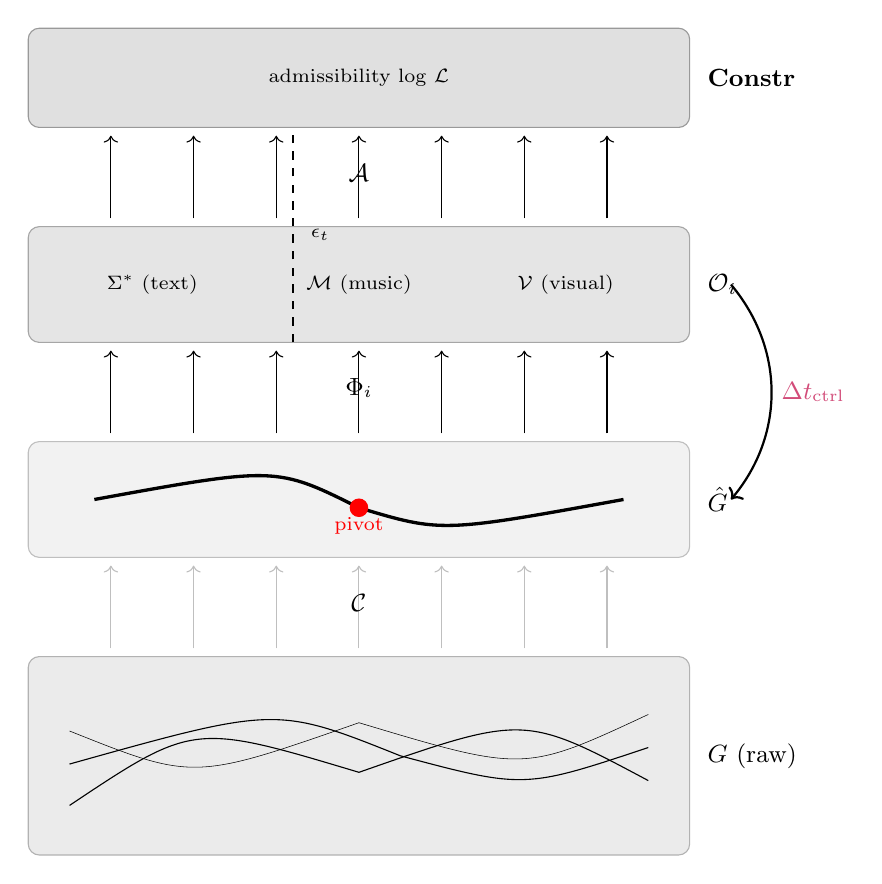
\begin{tikzpicture}[scale=1.05, every node/.style={font=\small}]

%% Layer 0: Raw gesture space G
\fill[black!8,draw=black!30,rounded corners=4pt]
  (-4,-1.2) rectangle (4,1.2);
\node[right] at (4.1,0) {$G$ (raw)};
% Noisy trajectories
\draw[thin]
  (-3.5,-0.6) .. controls (-2,0.4) .. (0,-0.2) .. controls (2,0.5) .. (3.5,-0.3);
\draw[very thin]
  (-3.5, 0.3) .. controls (-2,-0.3) .. (0, 0.4) .. controls (2,-0.2) .. (3.5, 0.5);
\draw[thin]
  (-3.5,-0.1) .. controls (-1, 0.6) .. (0.5,0.0) .. controls (2,-0.4) .. (3.5, 0.1);

%% Canonicalisation arrows (fibers)
\foreach \x in {-3,-2,-1,0,1,2,3}{
  \draw[->,gray!50] (\x, 1.3) -- (\x, 2.3);
}
\node at (0,1.85) {$\mathcal{C}$};

%% Layer 1: Canonical gesture space G-hat
\fill[black!5,draw=black!25,rounded corners=4pt]
  (-4,2.4) rectangle (4,3.8);
\node[right] at (4.1,3.1) {$\hat{G}$};
% Single clean canonical trajectory
\draw[very thick]
  (-3.2,3.1) .. controls (-1,3.5) .. (0,3.0) .. controls (1,2.7) .. (3.2,3.1);
\filldraw[red] (0,3.0) circle (3pt);
\node[below,red,font=\scriptsize] at (0,3.0) {pivot};

%% Projection arrows
\foreach \x in {-3,-2,-1,0,1,2,3}{
  \draw[->] (\x, 3.9) -- (\x, 4.9);
}
\node at (0,4.45) {$\Phi_i$};

%% Layer 2: Output space O_i
\fill[black!10,draw=black!35,rounded corners=4pt]
  (-4,5.0) rectangle (4,6.4);
\node[right] at (4.1,5.7) {$\mathcal{O}_i$};
\node[font=\scriptsize] at (-2.5,5.7) {$\Sigma^*$ (text)};
\node[font=\scriptsize] at ( 0.0,5.7) {$\mathcal{M}$ (music)};
\node[font=\scriptsize] at ( 2.5,5.7) {$\mathcal{V}$ (visual)};

%% Admissibility arrows
\foreach \x in {-3,-2,-1,0,1,2,3}{
  \draw[->] (\x, 6.5) -- (\x, 7.5);
}
\node at (0,7.05) {$\mathcal{A}$};

%% Layer 3: Constraint space
\fill[black!12,draw=black!40,rounded corners=4pt]
  (-4,7.6) rectangle (4,8.8);
\node[right] at (4.1,8.2) {$\mathbf{Constr}$};
\node[font=\scriptsize] at (0,8.2) {admissibility log $\mathcal{L}$};

%% Obstruction example
\draw[thick,dashed] (-0.8,5.0) -- (-0.8,7.6);
\node[right,font=\scriptsize] at (-0.7,6.3) {$\epsilon_t$};

%% Control loop (feedback from output back to canonical)
\draw[->,thick,bend left=40]
  (4.5,5.7) to node[right,purple!70]{$\Delta t_{\mathrm{ctrl}}$} (4.5,3.1);

\end{tikzpicture}
\caption{Unified geometric structure of the gesture-first framework.
Bottom to top: raw gesture space $G$; canonical space $\hat{G}$ (fibers
collapse under $\mathcal{C}$); output space $\mathcal{O}_i$ (lifted by
$\Phi_i$); constraint space $\mathbf{Constr}$ (evaluated by $\mathcal{A}$,
logged in $\mathcal{L}$). The dashed line shows an obstruction $\epsilon_t$
propagating through layers. The purple feedback arc represents the
control loop $\Delta t_{\mathrm{ctrl}}$ by which gesture can modify the
trajectory during projection.}
\label{fig:master}
\end{figure}

\FloatBarrier

% -------------------------------------------------------
\begin{thebibliography}{99}

\bibitem{wobbrock2007}
Jacob O. Wobbrock, Andrew D. Wilson, and Yang Li.
\newblock Gestures without libraries, toolkits or training: A \$1 recognizer
  for user interface prototypes.
\newblock In \emph{Proceedings of UIST}, 2007.

\bibitem{zhai2012}
Shumin Zhai and Per Ola Kristensson.
\newblock The word-gesture keyboard: Reimagining keyboard interaction.
\newblock \emph{Communications of the ACM}, 55(9), 2012.

\bibitem{killourhy2009}
Kevin S. Killourhy and Roy A. Maxion.
\newblock Comparing anomaly-detection algorithms for keystroke dynamics.
\newblock In \emph{Proceedings of DSN}, 2009.

\bibitem{monrose2000}
Fabian Monrose and Aviel D. Rubin.
\newblock Keystroke dynamics as a biometric for authentication.
\newblock \emph{Future Generation Computer Systems}, 16(4), 2000.

\bibitem{gunetti2005}
Daniele Gunetti and Claudia Picardi.
\newblock Keystroke analysis of free text.
\newblock \emph{ACM Transactions on Information and System Security}, 8(3),
  2005.

\bibitem{plover}
The Plover Project.
\newblock Open-source stenography software, 2010--present.
\newblock \url{https://www.openstenoproject.org/plover/}

\bibitem{mackenzie2002}
I.~Scott MacKenzie and R.~William Soukoreff.
\newblock Text entry for mobile computing: Models and methods, theory and
  practice.
\newblock \emph{Human-Computer Interaction}, 17(2--3), 2002.

\bibitem{schieber2001}
Marc H. Schieber.
\newblock Individuated finger movements: Limb kinematics, physiology, and motor
  control.
\newblock \emph{Journal of Neurophysiology}, 2001.

\bibitem{lashley1951}
Karl Lashley.
\newblock The problem of serial order in behavior.
\newblock In \emph{Cerebral Mechanisms in Behavior}, 1951.

\bibitem{lumatone}
Lumatone Music.
\newblock Lumatone isomorphic keyboard documentation, 2021.
\newblock \url{https://www.lumatone.io/}

\bibitem{juarrero1999}
Alicia Juarrero.
\newblock \emph{Dynamics in Action: Intentional Behavior as a Complex System}.
\newblock MIT Press, 1999.

\bibitem{juarrero2002}
Alicia Juarrero.
\newblock Context changes everything: How constraints create coherence.
\newblock \emph{Emergence}, 4(1--2):99--110, 2002.

\bibitem{cox2016}
Arnie Cox.
\newblock \emph{Music and Embodied Cognition: Listening, Moving, Feeling, and
  Thinking}.
\newblock Indiana University Press, 2016.

\bibitem{needham1997}
Tristan Needham.
\newblock \emph{Visual Complex Analysis}.
\newblock Oxford University Press, 1997.

\bibitem{cheng2025clio}
Newman Cheng, Gordon Broadbent, and William Chappell.
\newblock Cognitive loop via in-situ optimization: Self-adaptive reasoning for
  science.
\newblock arXiv:2508.02789, 2025.
\newblock \url{https://arxiv.org/abs/2508.02789}

\bibitem{iverson2005gesture}
Jana M. Iverson and Susan Goldin-Meadow.
\newblock Gesture paves the way for language development.
\newblock \emph{Psychological Science}, 16(5):367--371, 2005.

\bibitem{goldin2003gesture}
Susan Goldin-Meadow.
\newblock \emph{Hearing Gesture: How Our Hands Help Us Think}.
\newblock Harvard University Press, 2003.

\bibitem{savage2000ape}
E.~Sue Savage-Rumbaugh, Stuart G. Shanker, and Talbot J. Taylor.
\newblock \emph{Apes, Language, and the Human Mind}.
\newblock Oxford University Press, 2000.

\end{thebibliography}

\end{document}
